%% \chapter{\;\;\;\;Compiler Verification: CompCertM} %%이러면 (toc 말고 본문에서) 넘침
\chapter{\;\;\;\;Compiler Verification}
\label{sec:compiler}

We first give background on \cc{} and \ccc{}'s interaction semantics (\Cref{sec:compiler:background}), discuss the problems with interaction semantics (\Cref{sec:compiler:problems}) and present how we fixed it (\Cref{sec:compiler:solution}).
We show the flexibility of our framework by adding an advanced optimization (\Cref{sec:compiler:advanced}), and report our overall results in (\Cref{sec:compiler:compcertm}).
In \Cref{sec:compiler:semantics,sec:compiler:technique,sec:compiler:compcertr}, we flesh out formal details of our development.
Finally, we discuss related works in \Cref{sec:compiler:related}.
%% Finally, we discuss related works (\Cref{sec:compiler:related}).


\section{Background}
\label{sec:compiler:background}

\subsection{A Brief Introduction on CompCert}

\myparagraph{Undefined Behavior}



\section{Problems}
\label{sec:compiler:problems}

The problems with the interaction semantics of \ccc{} are that it does
not satisfy two adequacy properties. First, the adequacy w.r.t. C says
that for any C modules $M_1,\ldots,M_n$, the behaviors of the linked
program according to interaction semantics $\beh{M_1 \llink
  \ldots \llink M_n}$ should \emph{be included in} those according to the
physical semantics $\beh{M_1 \plink \ldots\plink M_n}$.  The reason for
failure was quite simple and we could easily fix it: unlike \ccc{}, we allow passing
the \texttt{undef} value to an external module since the C semantics
does so, while we turn ill-typed values into \texttt{undef} when they
are passed to an external module.

Second, the failure of the adequacy w.r.t. assembly is more serious.
Adequacy says that for any assembly modules $M_1,\ldots,M_n$,
the behaviors of the linked program according to interaction
semantics $\beh{M_1 \llink \ldots \llink M_n}$ should \emph{include}
those according to the physical semantics $\beh{M_1 \plink \ldots\plink M_n}$.
Note that the direction is opposite since assembly is the target language.
As discussed before, the reason for failure is that
the interaction semantics of \ccc{} does not have a mechanism to detect
illegal interference and make it undefined behavior~(UB).

\section{Solution}
\label{sec:compiler:solution}

We identify the sources of inadequacy w.r.t. assembly as violations of
three assumptions made by standard compilers: two on the registers and one on the stack.
We discuss why they 
cause problems with counterexamples and show how to semantically
handle them without changing the underlying language semantics.

\subsection{Assumptions on the Registers}
\label{sec:overview-semantics-register}
%
The two problematic assumptions on the registers are that
an invoked assembly function $(i)$ should
preserve the initial values of the callee-save registers, and $(ii)$
should not access the memory via the leftover pointer values remaining
in those registers that are not involved in passing meaningful information to the callee,
which we henceforth call \emph{\nip{}} registers.
%% in those registers, which we call \emph{non-passing} registers,
%% that are not involved in passing information to the callee.
%% the \emph{non-passing} registers (\ie those registers not involved
%% in passing information to the callee).
%% We discuss these two conventions together because it is nontrivial to find a
%% single model that enforces both conventions at the same time.
%% \jeehoon{I don't understand the last sentence..}
%% \jeehoon{``\nip{}'': how about ``opaque''?}

\begin{figure}[t]
\fbox{\begin{minipage}{.9pc}\mbox{}\\[15.25mm](a)\\[13.45mm]\mbox{}\end{minipage}}
\hspace*{-2.7mm}
\begin{minipage}{0.70\textwidth}
\begin{Verbatim}[frame=single]
int main()   {          main:
  int* x = malloc(8);     ...
  x[0] = 0;               *(%rbx) = 0;
  x[1] = 1;               *(%rbx + 4) = 1;
  f();               -->  f();
  out(x[0]);              out(*(%rbx));
  ...                     ...
}
\end{Verbatim}
\end{minipage}
$\mbox{}~\mathlarger{\mathlarger{\mathlarger{\mathlarger{\mathlarger{\llink}}}}}~\mbox{}$
\\
\vspace{3mm}
\\
\fbox{\begin{minipage}{.9pc}\mbox{}\\[10.50mm](b)\\[8.70mm]\mbox{}\end{minipage}}
\hspace*{-2.7mm}
\begin{minipage}{0.33\textwidth}
\begin{Verbatim}[frame=single]
f:
  if (g(%rbx))
    %rbx = %rbx + 4;
  else
    *(%rbx) = 1;

\end{Verbatim}
\end{minipage}
\caption{A counterexample showing the problem with the assumptions on the registers}
\label{fig:reg-convention}
\end{figure}

\myparagraph{Counterexamples}
%
The example in \Cref{fig:reg-convention} shows how violations of the two
assumptions can invalidate correct compiler translations.
%% \jeehoon{I think counterexample should go to the problems section.}
%
The code in the left box~(a) shows a standard translation of C code into assembly
(written in pseudocode) performed by mainstream compilers like GCC and LLVM, where the accesses to
the array \texttt{x} are translated into accesses via the register
\texttt{\%rbx} assuming that \texttt{\%rbx} is set to contain the
address of \texttt{x}. An important point here is that the compiler
assumes that $(i)$ the value of \texttt{\%rbx} is unchanged across
the function call \texttt{f()} since it is a callee-save register,
and also $(ii)$ the values in the array pointed to by \texttt{\%rbx} are
unchanged across \texttt{f()} since the array's addresses do not escape
except via \nip{} registers like \texttt{\%rbx}.
Therefore, the compiler expects that \texttt{out(*(\%rbx))} in the target code
correctly outputs \texttt{0}.

The right box~(b) presents an example of handwritten assembly
(written in pseudocode) for function \texttt{f} that violates the
above two assumptions of the compiler. The code either increments
\texttt{\%rbx} by \texttt{4} or writes \texttt{1} to \texttt{*(\%rbx)}
depending on the result of call to \texttt{g}.  Now if we link the assembly
code in (a) and that in (b) together, one can easily see that
\texttt{out(*(\%rbx))} incorrectly outputs~\texttt{1} instead
of \texttt{0} in either case: in the former case, \texttt{\%rbx}
points to the second element of the array~\texttt{x}, which contains
\texttt{1}; in the latter case, the value of \texttt{*(\%rbx)} is
directly updated to \texttt{1}. Therefore, it makes sense to
define those illegal behaviors of (b) as undefined behavior~(UB).

\myparagraph{Our Model}
\label{sec:compiler:solution:model}
%
We present our model making the illegal behaviors UBs
in stages, explaining at each stage why naive models do not work.
%% \jeehoon{What's the difference between ``stage'' and ``state''?}
%% \jeehoon{We have ``Our Solution'' paragraph inside ``Our Solution'' section. How about moving
%%   counterexample to the problems section, and giving a paragraph to each stage?}

First, in order to enforce the preservation of callee-save register
values, we store the initial values of the callee-save registers at
the \texttt{init-core} step of assembly modules; and check, at the
\texttt{halted} step, whether the final values of those registers are
equal to the stored initial values and if not, raise UB.  Here, the
question is, when a new core with a fresh register file is pushed into the core stack,
what values should be set as initial values of the \nip{}
registers including all of the callee-save registers.  Since the
registers may contain arbitrary values in the physical assembly
semantics, a natural choice would be to initially set them to contain
the \texttt{undef} value, which is an abstract value representing all
possible values. Indeed, this is the choice of \ccc{}.  However, there
is a serious problem. Since, for instance, \texttt{undef + 4} results
in \texttt{undef}, checking whether the final values of callee-save
registers are equal to the initial values, \ie \texttt{undef}, is
not sufficient. Specifically, the assembly code in (b) above
does not raise UB in this new semantics in case \texttt{g(\%rbx)} returns \texttt{1}
because the initial and final values of \texttt{\%rbx}
are both \texttt{undef} and thus equal
even though the callee-save register \texttt{\%rbx} is incremented
by \texttt{4} in the physical semantics.

Second, another natural solution would be to initially set the
\nip{} registers to nondeterministically contain arbitrary
values including \texttt{undef}. Though this model is more flexible,
it still has a problem. For instance, in the above example, to
simulate the physical behaviors of the assembly function \texttt{f} in
interaction semantics, one can set the initial value of \texttt{\%rbx} to
be either $(i)$ \texttt{undef} (\ie a more abstract value than the physical one), or
$(ii)$ a pointer to the array \texttt{x} (\ie a value equivalent to the physical one):
other values cannot be used since they are not refined by the value of \texttt{\%rbx} in the target,
which is required since the value is passed to an unknown function~\texttt{g}.
In the former case, if
\texttt{g(\%rbx)} returns \texttt{1}, we have the same problem with
callee-save checking as shown above.  In the latter case, if
\texttt{g(\%rbx)} returns \texttt{0}, the function \texttt{f}
successfully updates the array~\texttt{x} thereby invaliding the
translation in (a) as illustrated above.

We solve this problem by further revising the second model:
nondeterministically allocating an arbitrary number of \emph{junk
  blocks} (\ie blocks of size zero) and then initializing the
\nip{} registers with arbitrary non-pointer values or
\emph{junk pointers} (\ie pointers to the junk blocks).  Then we can
simulate the physical behaviors by initializing each register $r$
$(i)$ with the same non-pointer value if the physical value of $r$ is
a non-pointer value; and $(ii)$ otherwise with a fresh junk pointer.
The high-level idea is that, like \texttt{undef}, a junk pointer is
more abstract (\ie causing more UBs) than any pointer but, unlike
\texttt{undef}, sufficiently distinguishable. For instance,
in the previous example, if \texttt{g(\%rbx)} returns \texttt{1},
the initial and final values of \texttt{\%rbx} (\ie $p$ and $p+4$ for a junk pointer $p$)
are distinguished thereby raising UB by the callee-save checking;
if \texttt{g(\%rbx)} returns \texttt{0},
the memory access \texttt{*(\%rbx) = 1} raises UB because \texttt{\%rbx}
points to a junk block of size zero.

Finally, note that introducing nondeterminism as above is not a
showstopper thanks to the mixed simulation, as discussed in
\Cref{sec:overview-verification:mixedsim}: we can do forward
simulation everywhere except for the \texttt{init\_core} step of
assembly modules, where we should do backward simulation.

\subsection{Assumptions on the Stack}
\label{sec:overview-semantics-memory}
%
The problematic assumption on the stack is that the
\emph{outgoing arguments area} of a caller's stack (\ie where overflowing function
arguments are stored) should be fully \emph{owned} by the callee. In
other words, the callee can assume that the arguments area is never
modified by others unless its addresses are revealed to the public by
the callee itself.

\begin{figure}[t]
\fbox{\begin{minipage}{.9pc}\mbox{}\\[10.45mm](a)\\[8.65mm]\mbox{}\end{minipage}}
\hspace*{-1.9mm}
\begin{minipage}{0.255\textwidth}
  \begin{Verbatim}[frame=single]
main:
  ...  
  leak = %rsp;
  f(..., 0);
g:
  *leak = 1;
  \end{Verbatim}
\end{minipage}
$\mbox{}~\mathlarger{\mathlarger{\mathlarger{\mathlarger{\mathlarger{\llink}}}}}~\mbox{}$
\fbox{\begin{minipage}{.9pc}\mbox{}\\[10.45mm](b)\\[8.65mm]\mbox{}\end{minipage}}
\hspace*{-1.9mm}
\begin{minipage}{0.695\textwidth}
  \begin{Verbatim}[frame=single]
void f(..., int64_t x)       f:
{                              ...
  out(x);                      out(*(%rax));
  g();                  -->    g();
  out(x);                      out(*(%rax));
}                              ...
  \end{Verbatim}
\end{minipage}
\\[1mm]
\fbox{\begin{minipage}{.9pc}\mbox{}\\[15.90mm](c)\\[15.10mm]\mbox{}\end{minipage}}
\hspace*{-2.7mm}
\begin{minipage}{.95\textwidth}
\fbox{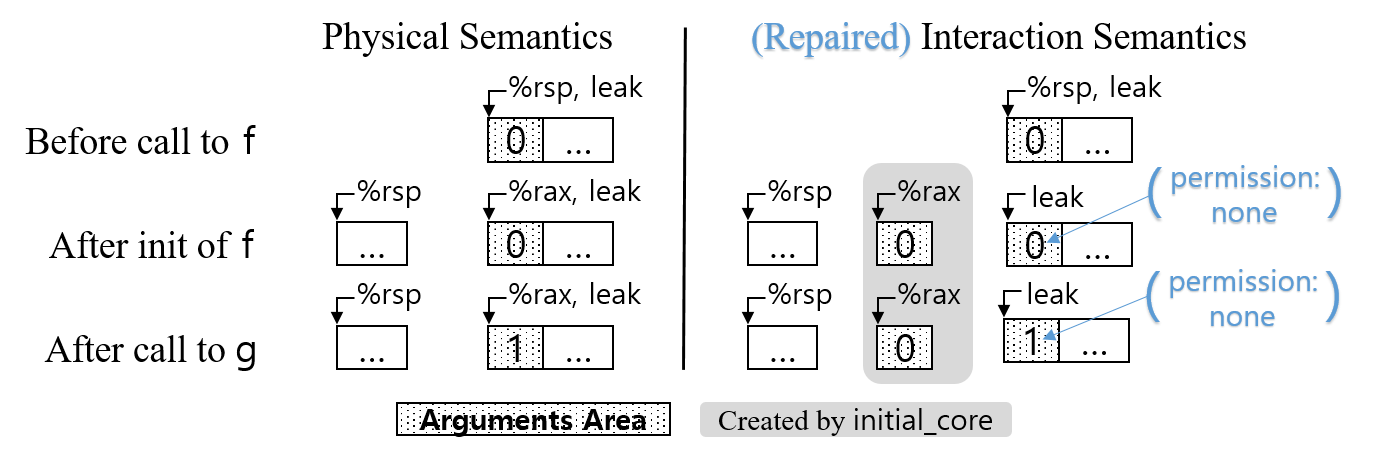
\includegraphics[width=.983\textwidth]{images/ex-stack.png}}
\end{minipage}
%% \fbox{\begin{minipage}{.8pc}\mbox{}\\[4.53mm](c)\\[3.73mm]\mbox{}\end{minipage}}
%% \hspace*{-1.9mm}
%% \begin{minipage}{.95\textwidth}
%%   \begin{Verbatim}[frame=single]
%%                      Physical Semantics         Interaction Semantics
%%                             %rsp           |                  %rsp       
%% Before call to f:           [=0=| ... ]    |                  [=0=| ... ]
%%                     %rsp    %rax           |    %rsp    %rax             
%%  After init of f:   [ ... ] [=0=| ... ]    |    [ ... ] [=0=] [=0=| ... ]
%%                     %rsp    %rax           |    %rsp    %rax             
%%  After call to g:   [ ... ] [=1=| ... ]    |    [ ... ] [=0=] [=1=| ... ]
%%   \end{Verbatim}
%% \end{minipage}
\caption{A counterexample showing the problem with the assumption on the stack}
\label{fig:stack-convention}
\end{figure}

\myparagraph{Counterexamples}
%
The example in \Cref{fig:stack-convention} shows how violations of the assumption
can invalidate correct compiler translations.
%
The box~(a) shows handwritten assembly code implementing two functions
\texttt{main} and \texttt{g}; the box~(b) shows a standard translation
of C code into assembly essentially performed by \texttt{gcc -O0}; and
the left-hand side (LHS) of the box~(c) depicts the shape of the stack
during execution in the physical semantics.
The function \texttt{main} stores the address of the
outgoing arguments area (\ie \texttt{\%rsp} as depicted in LHS of (c))
in the global variable \texttt{leak} and invokes the function
\texttt{f}, where the last argument \texttt{0} is stored in the
arguments area of the stack. Then the function \texttt{f} makes three
function calls, \texttt{out(x)}, \texttt{g()} and \texttt{out(x)},
where the argument \texttt{x} is directly read from the arguments area
pointed to by \texttt{\%rax} in the assembly, as depicted in LHS of
(c), and \texttt{out(x)} outputs the read value.  Finally, the
function \texttt{g} updates the arguments area pointed to by
\texttt{leak} with~\texttt{1}, as depicted in LHS of (c), between the
two function calls \texttt{out(x)}.

An important point here is that the compiler assumes that the
arguments area (\ie \texttt{\%rax}) is unchanged across the
function call \texttt{g()} since it is fully owned by \texttt{f}.
Therefore, the compiler expects that both calls
\texttt{out(*(\%rax))} in the target code correctly output
\texttt{0}. However, since the function \texttt{g} updates the
arguments area with \texttt{1} via \texttt{leak}, the two calls
incorrectly output \texttt{0} and~\texttt{1}.
We confirmed this incorrectness by
compiling \texttt{f} with \texttt{gcc -O2}, which
eliminates the second load \texttt{*(\%rax)} by propagating
the result of the first load across \texttt{g()}
thereby outputting \texttt{0} twice.

\myparagraph{Our Model}
%
In order to solve the problem, we have to distinguish accesses to the
arguments area via the caller from those via the callee and define the
former as UB. Though making such distinction is difficult in the
physical semantics, fortunately it is already made in interaction
semantics due to the language-independent design. For example, consider
the interaction semantics of the above example, depicted in the
right-hand-side (RHS) of \Cref{fig:stack-convention}~(c).  The
difference is that when the assembly function \texttt{f} is invoked,
the initialization process (\ie \texttt{init\_core}) of the module
semantics newly constructs the arguments area of the stack from the
given logical arguments in order to make an environment needed to
execute the assembly function \texttt{f}. This is essentially needed
because the caller may not be an assembly module so that it may not
have its own stack at all.  Then the callee sees the new arguments
area created by \texttt{init\_core} while the caller (in assembly)
sees the original arguments area.

Although the original interaction semantics does not prevent access to
the arguments area via the caller, we can easily fix it.
%% Now we can easily repair the original interaction semantics to make
%% those accesses to the arguments area via the caller as UB during the
%% lifetime of the callee.
We simply $(i)$ turn off the access
permission of the original arguments area in the \texttt{at\_external}
step of the caller module, and $(ii)$ turn it back on in the
\texttt{after\_external} step. Note that the notion of permission
%% is already an existing feature of
already exists in the \cc{} semantics, so that we do not
need to strengthen it. In the above example again,
the update by \texttt{g} will raise UB since the original argument area pointed
to by \texttt{leak} has no access permission.


\subsection{Mixed Simulation}
\label{sec:overview-verification:mixedsim}

While the target language of \cc{} is deterministic (more precisely,
the source is receptive and the target is determinate) thereby mostly
using forward simulations, the repaired interaction semantics of
\ccm{} is inherently nondeterministic to handle illegal interference from assembly modules
%% enforce the assembly calling conventions
(\Cref{sec:compiler:solution:model}) thus preventing the
use of forward simulation.
%% While it is theoretically possible to convert the \cc{}
%% verification from forward to backward simulations, it would incur a
%% significant cost since a compiler pass typically compiles a single
%% instruction in the source down to several instructions in the target.
%% %% due to the nature of source and target languages and the size of verification.
%% For this reason, determinism
%% has been considered ``instrumental for the simulation proofs of the compiler passes and its absence
%% is a show stopper''~\cite{besson:intptr}.
% Extending \cc{}'s semantics with such nondeterministic features can potentially cause significant
% overhead, as it invalidates forward simulation and enforces one to use backward simulation, which
% effectively means one should re-establish simulation proof from the scratch.  In literature, it is
% even said that

In order to recover the ability to use forward simulation in the occasional presence of nondeterminism,
we adopt the idea of \emph{mixed (forward-backward) simulation} from \cite{neis:pilsner}.
%% To embrace nondeterminism with low verification cost, we develop more general simulations, called
%% \emph{mixed simulations}, that (mostly) allow forward reasoning in the (occasional) presence of
%% nondeterminism.
The key observation is that
the requirement for using forward simulations (\ie determinism of the target) is a per-state property,
not a per-language property: as long as a particular target machine state is \emph{locally deterministic} (\ie its next state is unique),
one can do forward simulation at that state.
%% conversion from backward to forward simulations
%% requires only the current target \emph{machine state}, not the entire target \emph{language}, to be
%% deterministic.
Based on this observation, mixed simulations selectively allow forward
simulation when the target is locally deterministic, in addition to
the default backward simulation.
%% for each pair of related machine states, we allow the verifier to
%% \emph{choose} to perform either forward or backward reasoning, requiring that forward reasoning is
%% used only for locally deterministic target machine states.
%
Specifically, we say that a relation $R$ is a (closed) mixed simulation if
for all $(\mssrc, \mstgt) \in R$,
%% \makebox[\linewidth]{\makebox[1.2\linewidth]{
%% \begin{minipage}{1.2\linewidth}
\begin{enumerate}
\item
  $\forall e, \mstgt',~ \mstgt \estep{e} \mstgt' \implies {} $ \\
  $ \exists \mssrc',~ \mssrc \estep{\tau}^{\raisebox{-1mm}{\scriptsize$\ast$}} \estep{e}\estep{\tau}^{\raisebox{-1mm}{\scriptsize$\ast$}} \mssrc' \land (\mssrc', \mstgt') \in R$; or
\item
  $\forall e, \mssrc',~ \mssrc \estep{e} \mssrc' \implies {} $ \\
  $ \exists \mstgt',~ \mstgt \eustep{\tau}^{\raisebox{-1mm}{\scriptsize$\ast$}} \eustep{e}\eustep{\tau}^{\raisebox{-1mm}{\scriptsize$\ast$}} \mstgt' \land (\mssrc', \mstgt') \in R$\\
\end{enumerate}
%% \end{minipage}
%% }}
where $\ms \eustep{e} \ms'$ denotes that $\ms$ is locally deterministic and $\ms \estep{e} \ms'$.

\Cref{fig:mixedsim} visualizes this formulation of mixed simulation, where
%% presents an example of mixed simulations, where $R$ is a simulation relation; red and blue circle represent source and
%% target machine states, respectively;
solid and dotted arrows represent universally and existentially
quantified steps, respectively, and double circles represent locally
deterministic target states. In this figure,
since the first three target machine states are deterministic,
we can do forward simulation as shown in the figure;
then, since the following target state is nondeterministic,
we should do backward simulation as shown in the figure.
%% the first three target machine states are deterministic.  The
%% first three target steps are deterministic and reasoned in a forward manner (from source to target),
%% and the last target step is nondeterministic and reasoned in a backward manner (from target to
%% source).  Later, those part of simulations that are reasoned in a forward manner is converted to
%% backward reasoning, thereby proving backward simulation and thus behavior refinement.

Note that the repaired interaction semantics is nondeterministic only
at the initial step of a module invocation, so that we can do
forward simulation everywhere else using mixed simulations.

In order to support \cc{}'s condition for forward simulation,
we also add the following to the above formulation of mixed simulation:
\begin{enumerate}[resume]
\item or, $\mssrc$ is receptive and\\
  $\forall e, \mssrc',~ \mssrc \estep{e} \mssrc' \implies {} $ \\
  $ \exists \mstgt',~ \mstgt \exstep{\tau}^{\raisebox{-1mm}{\scriptsize$\ast$}} \exstep{e}\exstep{\tau}^{\raisebox{-1mm}{\scriptsize$\ast$}} \mstgt' \land (\mssrc', \mstgt') \in R$\\
  where $\ms \exstep{e} \ms'$ denotes that $\ms$ is locally determinate and $\ms \estep{e} \ms'$.
\end{enumerate}
Also we apply this mechanism of mixed simulation to our open simulations.

\begin{figure}[t]%% {0.43\textwidth}
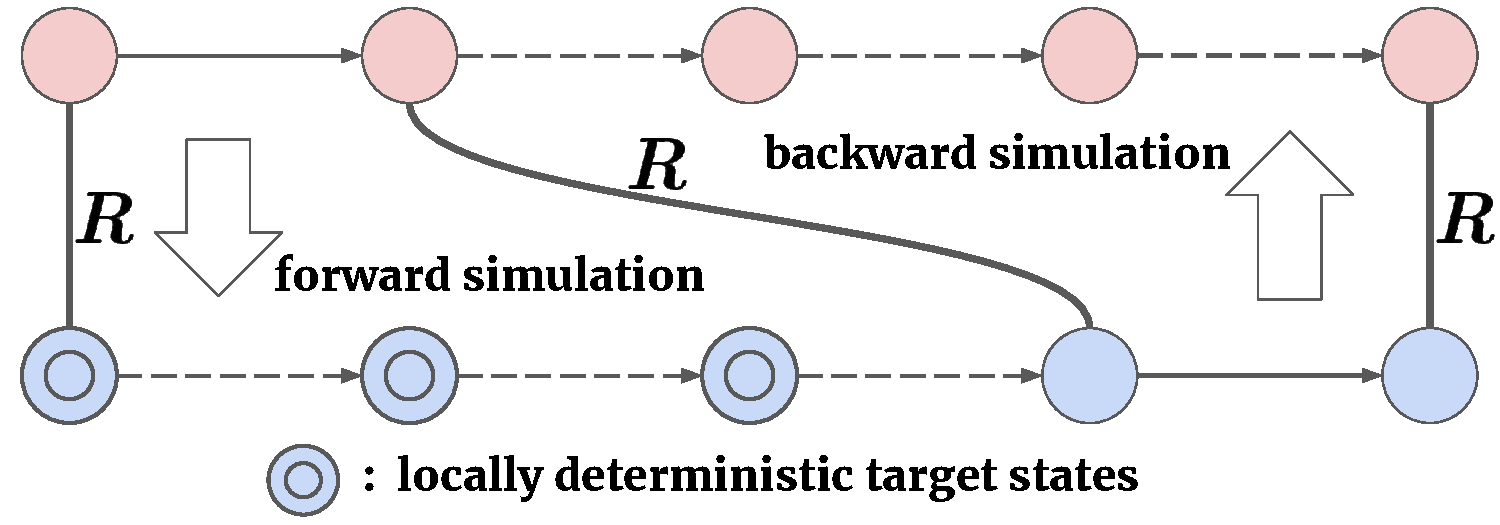
\includegraphics[width=0.7\textwidth]{images/mixed-sim-bold.pdf}
%% 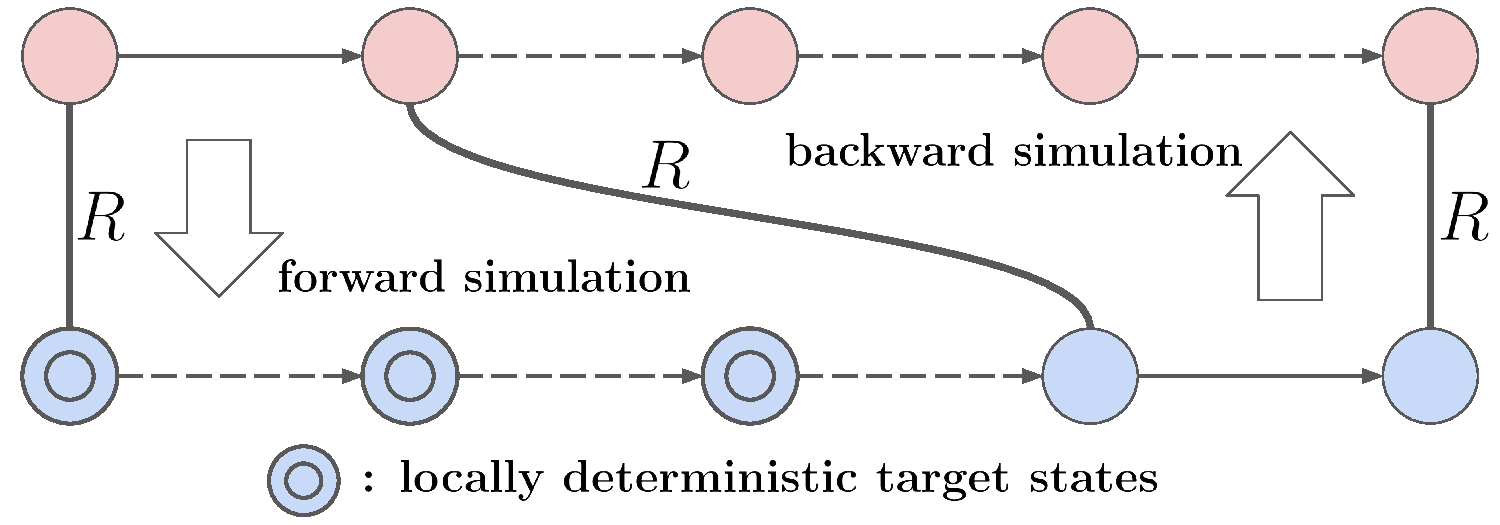
\includegraphics[width=0.7\textwidth]{images/mixed-sim.pdf}
\caption{A visualized example of mixed simulations}
\label{fig:mixedsim}
\end{figure}

\section{Advanced Optimizations with Module-Local Invariants}
\label{sec:compiler:advanced}

To demonstrate the flexibility of our framework -- allowing arbitrary memory relations -- we added a new optimization, \texttt{Unreadglob}, whose verification requires a new memory relation.
We flesh out the details in the following order: first we present {\it enriched memory injection}, a mildly strengthened version of \cc{}'s original injection (\Cref{sec:overview-verification:injection:static}),
then the new memory relation (\Cref{sec:overview-verification:injection:dynamic}), and finally \texttt{Unreadglob} optimization (\Cref{sec:compiler:advanced:unreadglob}).
%% In this section, we present {\it enriched memory injection}, a mild generalization of \cc{}'s original injection (\Cref{sec:overview-verification:injection:static}),
%% the new memory relation \Cref{sec:overview-verification:injection:dynamic}, and \texttt{Unreadglob} optimization \Cref{fig:overview-modulelocal:compiler}.

%% In this section we present what our framework additionally offers about compiler and
%% program verification: verifying more advanced compiler optimizations with module-local
%% invariants (\Cref{sec:overview-modulelocal:compiler}) and verifying program modules against their
%% mathematical specification modules (\Cref{sec:overview-modulelocal:program} and \Cref{sec:overview-modulelocal:utod}).

\myparagraph{Enriched Memory Injection}
\label{sec:overview-verification:injection:dynamic}
%
For open modules, reasoning about dynamically allocated local memory
such as a function's stack frame requires to strengthen the original
memory injection due to the presence of unknown modules.  The reason
is because when reasoning about a module $M$, we have to assume that
an unknown function invoked by $M$ does not change the dynamic local
memory of $M$ and also guarantee that a function of $M$ invoked by an
unknown module does not change the caller's dynamic local memory.

For this purpose, \ccc{} introduces \emph{structured injections} that
enrich the original memory injections with ownership information (\ie
whether owned by the current module or others) for all memory blocks
including public ones.  Using them, structured simulations impose
fine-grained invariants subject to the ownership information and a
concrete leakage protocol based on reachability from pointers.

Unlike \ccc{}, \ccm{} generalizes open simulations and memory injections
in a more abstract way following \cite{DBLP:conf/icfp/DreyerNB10,pb}.

First, we generalize the external call case of the open simulation in \Cref{fig:open-sim}
by allowing \emph{private transitions}, denoted $\sqsupseteq_\weak$,
as follows (\textcolor{red}{in red color}):
\[
\begin{array}{@{}l@{}}
\texttt{ 5:}~\quad \textcolor{red}{\exists w' \sqsupseteq_\weak w},~ (f_\src,f_\tgt)\in \texttt{vrel}(\textcolor{red}{w'}) \land (\vec{v}_\src,\vec{v}_\tgt) \in \overrightarrow{\texttt{vrel}(\textcolor{red}{w'})} \land{} \\[1mm]
\texttt{ 6:}~\quad \textcolor{red}{\forall w'' \sqsupseteq w'},~\forall (\memsrc',\memtgt')\in\texttt{mrel}(\textcolor{red}{w''}),~ \forall (r_\src,r_\tgt)\in \texttt{vrel}(\textcolor{red}{w''}),\\[1mm]
\texttt{ 7:}~\quad \textcolor{red}{\exists w''' \sqsupseteq_\weak w'',~ w''' \sqsupseteq w} \land {} \\
\phantom{\texttt{ 7:}}~\quad ((\memsrc',\mathtt{after\_external}~r_\src~\stsrc),(\memtgt',\mathtt{after\_external}~r_\tgt~\sttgt))\in R(\textcolor{red}{w'''})
\end{array}
\]
Though private transitions are allowed before and after an external function call (\ie
$w' \sqsupseteq_\weak w$ and $w''' \sqsupseteq_\weak w''$),
the overall transition should be \emph{public} (\ie $w''' \sqsupseteq w$)
assuming the external call also makes a public transition (\ie $w'' \sqsupseteq w'$).%
\footnote{We only allow private transitions just before and after external calls for simplicity.
See \Cref{sec:related} for comparison with \cite{DBLP:conf/icfp/DreyerNB10,pb}.}

Second, we extend memory injections to specify others' dynamic local
memories in the source and target that should be unchanged by the current module.
Specifically, an (enriched) memory injection $(\iota, m^\weak_\src, m^\weak_\tgt)$
consists of an original memory injection $\iota$ mapping the source public blocks into target blocks; and additionally
a private (\ie dynamic local) memory of the source $m^\weak_\src$ and that of the target $m^\weak_\tgt$
where $m^\weak_\src$ and $m^\weak_\tgt$ should be disjoint from the public memories specified by~$\iota$.
Then, private transitions from $(\iota, m^\weak_\src, m^\weak_\tgt)$ to
$(\iota', {m'}^\weak_\src, {m'}^\weak_\tgt)$ only require that $\iota'$ should extend $\iota$,
while public transitions additionally require that private memories should be unchanged
(\ie $m^\weak_\src = {m'}^\weak_\src$ and $m^\weak_\tgt = {m'}^\weak_\tgt$).
Note that all the areas of the source and target memories that are not on $m^\weak_\src$, $m^\weak_\tgt$ or the injection map $\iota$
are considered as \emph{private} (\ie dynamic local) memory of the current module.

%% \begin{wrapfigure}{r}{0.45\textwidth}
\begin{minipage}{1\textwidth}
\mbox{}\\[-7mm]    
\begin{Verbatim}
   int f() {          int f() {     
1:   int a0;            int a[2];   
2:   reg a1 = 0;  -->   a[1] = 0;   
3:   g(&a0);            g(&a[0]);   
4:   return a1;         return a[1];
   }                  }
\end{Verbatim}
\mbox{}\\[-10mm]
\end{minipage}
%% \end{wrapfigure}
To show how it works,
we give an example mimicking register spilling
in the presence of address-taken stack variables.
Consider the transformation on the right, where
in the source a memory block for \texttt{a0} and a function-local register for \texttt{a1} are allocated and
the address of \texttt{a0} escapes to \texttt{g},
while in the target a single block for both \texttt{a[0]} and \texttt{a[1]}
is allocated and the address of the block escapes to \texttt{g}.
Here \texttt{a0} can be seen as an address-taken stack variable and \texttt{a1} a spilled register.
The key difference is that, in the source, \texttt{a1} cannot be accessed by
\texttt{g} since it is a function-local register
while, in the target, \texttt{a[1]} can be accessed via the address of \texttt{a[0]}.

We now show how the target \texttt{f} simulates the source \texttt{f}
by logically protecting \texttt{a[1]} from \texttt{g}.
Though we give an informal description here to help understanding,
the formal definition of an open simulation $R$ 
can be easily derived from the description.
At line~$\texttt{1}$, any world $w_0$ and
memories $(m_\src, m_\tgt)$ related at $w_0$ are given. We take a step
to line~$\texttt{2}$ by extending $w_0.\iota$ (\ie the public
injection of $w_0$) to map $\texttt{a0}$ to $\texttt{a[0]}$, say $w_1$,
which is a public transition. At line~$\texttt{2}$, we take a step
to line~$\texttt{3}$ without changing the world $w_1$.
At line~$\texttt{3}$, we first make a private transition from $w_1$
to $w_2$ by extending $w_1.m^\weak_\tgt$
%(\ie the private area of the target memory)
to include the memory chunk $\texttt{a[1]} = 0$.
Then we assume that \texttt{g} makes a public transition from $w_2$ to $w_3$
returning any memories related at $w_3$. Thanks to $w_2.m^\weak_\tgt = w_3.m^\weak_\tgt$,
we know that the chunk $\texttt{a[1]} = 0$ remains the same.
Then we make a private transition from $w_3$ to $w_4$ by
dropping the chunk $\texttt{a[1]} = 0$ from $w_3.m^\weak_\tgt$.
Since $w_4.m^\weak_\tgt = w_1.m^\weak_\tgt$, we have a public transition from $w_1$ to $w_4$.
Finally, at line~$\texttt{4}$, we know that both the register $\texttt{a1}$ and
the memory-allocated variable $\texttt{a[1]}$ contain
$\texttt{0}$ and thus the same value $\texttt{0}$ is returned.

It is important to note that the (others') private memories $w.m^\weak_\src$ and $w.m^\weak_\tgt$ of a
memory injection $w$ are preserved as long as a function accesses
$(i)$ the memory via public addresses, or $(ii)$ its own private memory.
In the former case,
since a public block of the source is fully injected into a block of the target,
%% ---this is why the mapping is called an injection---
whenever a pointer offset goes beyond the public area mapped by the injection $w.\iota$,
the source program accesses an unallocated area thereby raising UB.
In the example above, if \texttt{g} in the target accesses \texttt{*(\&a[0]+1)},
then in the source it accesses \texttt{*(\&a0+1)}, which raises UB.
In the latter case, since the function's own private memory
is disjoint from all the memories specified by~$w$,
accessing it does not affect $w$. In the example above, at line~\texttt{2} in the target, 
the assignment \texttt{a[1] = 0} preserves $w_1.m^\weak_\tgt$ (and also the target public memory of $w_1$) because we know that
the current private memory \texttt{a[1]} is disjoint from the area specified by $w_1$ by construction.

\newrevision{Also note that any part of the public memories cannot be
  converted to a private one since the injection map is only
  extended at each step; and any part of the others' private memories
  (\ie $m^\weak_\src$ and $m^\weak_\tgt$) cannot be
  converted to the current module's private one since all
  \emph{proper} steps (\ie local steps or steps across an external
  call) only allow public transitions (\ie preserving $m^\weak_\src$ and $m^\weak_\tgt$).}

%% $R(w)$ relates any memories related at $w$ and
%% we take a step to line~$\texttt{2}$ by extending $w.\iota$
%% (\ie the (public) injection of $w$)
%% to map $\texttt{a0}$ to $\texttt{a[0]}$. At line~$\texttt{2}$,
%% $R(w)$ requires that $w.\iota$ maps $\texttt{a0}$ to $\texttt{a[0]}$

%% We now show how to logically protect \texttt{a[1]} from \texttt{g} and
%% prove that the two programs are related by an open simulation $R$.
%% First, $R$ relates each corresponding line of \texttt{f} in the source
%% and target.  We will then explain, at each line, how $R$ relates
%% source and target memories and satisfies the open simulation property.
%% At line~$\texttt{1}$, $R(w)$ relates any memories related at $w$ and
%% we take a step to line~$\texttt{2}$ by extending $w.\iota$
%% (\ie the (public) injection of $w$)
%% to map $\texttt{a0}$ to $\texttt{a[0]}$. At line~$\texttt{2}$,
%% $R(w)$ requires that $w.\iota$ maps $\texttt{a0}$ to $\texttt{a[0]}$

%% First,
%% we define an open simulation $R(w)$ to relate any memories related at
%% $w$ and each corresponding line of \texttt{f} in the source and
%% target. Second, we prove that 

%% Explain open simulation

\myparagraph{Memory Injection with Module-Local Invariants}
\label{sec:overview-verification:injection:static}
%
For open modules, reasoning about statically allocated local memory
such as static variables of C requires a further generalization.  The
problem is that when an open module $M$ invokes an unknown function
$f$, one cannot assume that the static memory of $M$ is unchanged
during the call because $f$ may call back a function from $M$, which
may change the static memory. However, since the static memory is only
accessible to the known functions in $M$, one can find a certain
invariant on the static memory by analyzing all the functions of $M$
and expect that an external call preserves the invariant although the
static memory can be changed. Enabling such reasoning is simple:
\ccm{} just adds another component in a memory injection $w$ that
globally imposes a given invariant on selected static variables
disjoint from $w.m^\weak_\src$, $w.m^\weak_\tgt$ and $w.\iota$.
We give examples using module-local invariants in \Cref{sec:overview-modulelocal}.


\begin{figure}[t]
\begin{Verbatim}
static int x = 0;       static int x = 0;                   
int f() {               int f() {              int f() {    
  g();           [CP]     g();          [UG]     g();       
  x = 1;        ----->    x = 1;       ----->               
  return x;               return 1;              return 1;  
}                       }                      }            
\end{Verbatim}
\begin{Verbatim}
static int y = 0;
void g() {
  if (y == 0) {
    y = 1; f();
  }
}                 
\end{Verbatim}
\caption{An example of \texttt{Unreadglob} optimization}
\label{fig:overview-modulelocal:compiler}
\end{figure}

\myparagraph{Unreadglob Optimization}
\label{sec:compiler:advanced:unreadglob}
We developed a new optimization \texttt{Unreadglob} eliminating all
unread static variables and instructions writing to them.
\Cref{fig:overview-modulelocal:compiler} shows an example
optimization, where $(i)$ the first program is optimized to the second
one by constant propagation~(CP) replacing \texttt{return x} by
\texttt{return 1}; and $(ii)$ the second one is optimized to the third
one by \texttt{Unreadglob}~(UG) eliminating the unread static variable
\texttt{x} and the command \texttt{x = 1}.  It is important to note
that across the function call \texttt{g()}, the static variable
\texttt{x} may be updated from \texttt{0} to \texttt{1} because the
function \texttt{g} can indirectly update it by calling \texttt{f} as shown in
the fourth program in \Cref{fig:overview-modulelocal:compiler}.

\revision{In verification of the optimization \texttt{UG} above,
we have to use memory injections $w$ with module-local invariants
introduced in \Cref{sec:overview-verification:injection:static}.
The reason is that the static variable \texttt{x} in the source cannot reside
$(i)$ in the injection map $w.\iota$ since \texttt{x} does not exist in the target; or
$(ii)$ in the source private $w.m^\weak_\src$ since \texttt{x} can be modified
during the external call \texttt{g()}.
To verify \texttt{UG} above, we can impose the trivial invariant
\texttt{Top} on the eliminated static variable \texttt{x}, meaning
that \texttt{x} can be modified arbitrarily, which is sufficient
because \texttt{x} is unread.}

Note that \ccx{} may be
able to verify \texttt{Unreadglob} using memory injections because it
assumes no mutual dependency among modules, so that no static
variables can be accessed via external function calls, unlike the above
example with mutual recursion.

\section{CompCertM}
\label{sec:compiler:compcertm}

Based on the theories we presented so far, we develop \ccm{}, an extension of \cc{} with the
repaired interaction semantics and open simulations to support multi-language linking.  We state
\ccm{}'s compositional correctness results (\Cref{sec:results:compiler}) and evaluate its
verification efforts (\Cref{sec:results:evaluation}).  \ccm{} currently supports the x86 backend only.
We do not currently see any technical problem with supporting other architectures.

\subsection{Compositional Correctness}
\label{sec:results:compiler}

\ccm{} uses open simulations with three parameters:
memory relations, symbol relations and memory predicates
(see \Cref{sec:main-verification:opensim} for details).
It supports $(i)$ the memory relations discussed in \Cref{sec:overview-verification:injection}:
identity, extension and (enriched) injections with no or any given module-local invariant;
$(ii)$ two symbol relations: one for keeping identical symbols in the source and target
and the other for allowing elimination of global variables in the target (only allowed for memory injections), needed for \code{Unusedglob} and \code{Unreadglob};
$(iii)$ two memory predicates: one for no analysis and the other for the value analysis of \cc{}.

Let $\rels$ be the set of open simulations with all possible parameters.
To apply RUSC, we prove that the \ccm{} compiler $\mathcal{C}$ transforms the source module with
a series of passes that are independently verified using open simulations in $\rels$.
\begin{lemma}[Pass Correctness]\label{thm:results-passes}
  For any \textrm{Clight} module $S$ and \textrm{Asm} module $T$, if $\mathcal{C}(S) = T$, then
  there exist intermediate modules $M_0, M_1, \cdots, M_n$ such that:
  \begin{enumerate}
  \item $M_0 = S$ and $M_n = T$; and
  \item $\forall i \in [0,n),~ \exists R \in \rels,~ (M_i, M_{i+1}) \in R$~.
  \end{enumerate}
\end{lemma}

We also prove all \textrm{Clight} and \textrm{Asm} modules are self-related.
\begin{lemma}[Self-Relatedness]\label{thm:results-relatedness} For any \textrm{Clight} or \textrm{Asm}
  module $M$, we have $M \in \self{\rels}$.
\end{lemma}
\noindent
\revision{Note that
  since we define illegal interference from Asm
  (\ie causing different behaviors in the source and target) as undefined behaviors (UBs)
  as shown in \Cref{sec:compiler:solution},
  every Asm module can be self-related.}

From \Cref{thm:results-passes,thm:results-relatedness}, the RUSC relation for the compiler follows.
\begin{theorem} [Modular Correctness]\label{thm:results-modular}
  For any \textrm{Clight} module $S$ and \textrm{Asm} module $T$, if $\mathcal{C}(S) = T$:
  \[
    {S} \rusc_\rels {T} \quad\text{with}\quad S,T \in \self{\rels}~.
  \]
\end{theorem}

\noindent
This theorem provides a truly compositional correctness
thanks to the compositionality of RUSC (\Cref{thm:rusc}):
%% The fact that the source and target are related by RUSC
%% implies that they satisfy behavioral refinement by adequacy of RUSC, and moreover
the relation can be freely (\ie vertically or horizontally) composed with any verification using RUSC
including that against mathematical specifications.
As an example, the following compositional correctness follows.
\begin{corollary} [Compositional Correctness 1]\label{thm:results-compiler}
  Let $(S_1,T_1), \ldots, (S_n,T_n)$ be pairs of source and target modules.
  If each pair is either compiled (\ie $\mathcal{C}(S_i) = T_i$ with $S_i$ \textrm{Clight} and $T_i$ \textrm{Asm}), or a self-related context (\ie $S_i = T_i \in \self{\rels}$), then
  \[
    \beh{S_1 \llink \cdots \llink S_n} \supseteq \beh{T_1 \llink \cdots \llink T_n}~.
  \]
\end{corollary}
%
\noindent This correctness theorem is compositional in the sense that behavior is refined in the
presence of any self-related contexts such as arbitrary \textrm{Clight} and \textrm{Asm} modules
(\Cref{thm:results-relatedness}).





Note that \textrm{Clight}, not \textrm{\cc{} C}, is the source language in the above theorems.  One of the
reasons is that \textrm{Clight} is the source language for most verification frameworks based on
\cc{}, such as VST~\cite{VST}, \ccc{}, and \ccx{}.  More importantly, we found that
\textrm{\cc{} C} is incompatible with memory injections.  Specifically,
\textrm{\cc{} C} imposes a strict alignment requirement on memory blocks of size zero, which, however,
%% but the requirement
is not preserved by memory injections.
%% For this reason, we cannot achieve full horizontal compositionality
%% in the presence of both \textrm{\cc{} C} modules and compiler passes verified using memory injections.
In other words, \textrm{\cc{} C} modules are not always self-related by memory injections.\footnote{This problem
  would be solved if one strengthens memory injections with more strict alignment requirements.}

\myparagraph{Supporting \textrm{\cc{} C}}
However, we can still prove a compositional correctness (not modular correctness as in \Cref{thm:results-modular}) for \textrm{\cc{} C}
following \scc{}'s \emph{Level A} technique~\cite{kang:scc},
which exploits the fact that all \textrm{CompCert C} modules are transformed to \textrm{Clight} modules
by the same two passes.
Specifically, the first pass is verified using an open simulation with the memory identity
and the second pass with memory injections, as done in the original \cc{}.
Then the following lemma follows from horizontal compositionality and adequacy of
open simulations (with memory identity and injection) and transitivity of behavioral refinement.

\begin{lemma} [ClightGen Correctness]\label{thm:results-clightgen}
  Let $(S_1,T_1), \ldots, (S_n,T_n)$ be pairs of source and target modules.
  If each pair is either translated (\ie $\textrm{ClightGen}(S_i) = T_i$ with $S_i$ \textrm{\cc{} C} and $T_i$ \textrm{Clight}), or a self-related context (\ie $S_i = T_i \in \self{\rels}$), then
  \[
    \beh{S_1 \llink \cdots \llink S_n} \supseteq \beh{T_1 \llink \cdots \llink T_n}~.
  \]
\end{lemma}



By composing \Cref{thm:results-compiler}, \Cref{thm:results-clightgen} and \Cref{thm:results-relatedness}, we have the following theorem.
\begin{theorem} [Compositional Correctness 2]\label{thm:results-compiler2}
  Let $(S_1,T_1), \ldots, (S_n,T_n)$ be pairs of source and target modules.
  If each pair is either compiled (\ie $\mathcal{C}(S_i) = T_i$ with $S_i$ \textrm{\cc{} C} or \textrm{Clight} and $T_i$ \textrm{Asm}), or a self-related context (\ie $S_i = T_i \in \self{\rels}$), then
  \[
    \beh{S_1 \llink \cdots \llink S_n} \supseteq \beh{T_1 \llink \cdots \llink T_n}~.
  \]
\end{theorem}


\myparagraph{Adequacy w.r.t. Physical Semantics}


We show that the repaired interaction semantics is adequate w.r.t. the physical semantics of \cc{},
where the former uses the language-independent linking $\llink$ and the latter the syntactic linking $\plink$
concatenating modules of the same language.

We prove that the physical semantics refines the repaired interaction semantics for \textrm{Asm} modules
using a closed simulation of \cc{} with memory injections.
\begin{theorem}[Adequacy w.r.t. Assembly]\label{thm:results-adequacy-asm}
  Let $M_1, \cdots, M_n$ be \textrm{Asm} modules.  We have:
  \[   \beh{M_1 \llink \ldots \llink M_n} \supseteq  \beh{M_1 \plink \ldots \plink M_n} ~.\]
\end{theorem}
\noindent
\revision{This theorem allows us to carry verification results on the interaction semantics such as \Cref{thm:results-compiler2}
down to \cc{}'s Asm semantics with syntactic linking.}



Conversely, we prove that the repaired interaction semantics refines the physical semantics for \textrm{\cc{} C} modules
using a closed simulation of \cc{} with memory identity.
This result is useful because we want to allow separate compilation (of C modules) on the compiler side, and on the program verification side, we want to hide complexities from inter-module steps.
\begin{theorem}[Adequacy w.r.t C]\label{thm:results-adequacy-c}
  Let $M_1, \cdots, M_n$ be \textrm{\cc{} C} modules.  We have:
  \[  \beh{M_1 \plink \ldots \plink M_n} \supseteq \beh{M_1 \llink \ldots \llink M_n}  ~.\]
\end{theorem}


In some sense, the \Cref{thm:results-compiler2,thm:results-adequacy-asm,thm:results-adequacy-c} together forms a strong stress-test for a language-independent linking, and our results show strong evidence that our repaired interaction semantics is indeed adequate (in a literal sense).
Specifically, if one of the three desiderata is missing, it is trivial to find language-independent linking satisfying the others.
Without \Cref{thm:results-adequacy-asm}, one can define interaction semantics to always execute UB; then, the other theorems become trivial.
Without \Cref{thm:results-adequacy-c}, one can define the behavior of interaction semantics to an empty set.
Without \Cref{thm:results-compiler2}, one can define $\llink \defeq \plink$.

%% These results mean that the repaired interaction semantics does not give too few behaviors to assembly programs (e.g., missing physically observable behaviors), nor does it give too many behaviors to well-typed C programs (e.g., giving UB to them).


Interestingly, by composing \Cref{thm:results-compiler2,thm:results-adequacy-asm,thm:results-adequacy-c}, we obtain
the same separate compilation correctness result of \scc{}~\cite{kang:scc}:

\begin{corollary}[Separate Compilation Correctness]
  Let $S_1, \ldots, S_n$ be \textrm{\cc{} C} modules and $T_1, \ldots, T_n$ be \textrm{Asm} modules.
  If $\mathcal{C}(S_i) = T_i$ for each $i$, we have:
  \[
    \beh{S_1 \plink \cdots \plink S_n} \supseteq \beh{T_1 \plink \cdots \plink T_n}~.
  \]
\end{corollary}

\youngju{Just mention that \ccc{} does not satisfy upperbound, and explain it in appendix?}
\youngju{here? or appendix?: To this end, we have strengthened \cc{}'s type checker in a number of
  ways, ruling out trivially wrong (according to C standard) programs more than before.  We rule out
  (i) a program that contains an identifier that is not declared in the module (ii) ``return''
  (without value) statement used for non-void function (iii) ``return'' (with value) statement used
  for void function (iv) function arguments containing void type.  (v) has duplicate (function or
  global variable) identifiers (vi) A function argument with size bigger than INT\_MAX (\cc{}
  already aborts on such programs)}





\subsection{Evaluation of Verification Efforts}\label{sec:results:evaluation}

\begin{table}[t]
\footnotesize

\parbox{\linewidth}{
\caption{SLOC of \ccm{} and related works --- compared to its baseline \cc{}, respectively}
\begin{tabu}{@{}l@{\hspace{1.55pt}}|[1.25pt]@{\hspace{1.55pt}} c @{\hspace{1.55pt}}|@{\hspace{1.55pt}} c @{\hspace{1.55pt}}|@{\hspace{1.55pt}} c @{\hspace{1.55pt}}|[1.25pt]@{\hspace{1.55pt}} c @{\hspace{1.55pt}}|@{\hspace{1.55pt}} c @{\hspace{1.55pt}}|[1.25pt]@{\hspace{1.55pt}}}
Portion     & \shortstack{\cc{} \\ 3.5} & \ccr{} 3.5        & \ccm{} pack                                               & \shortstack{\cc{}\\ 2.1} & \ccc{} \\
\hline
Pass Proofs & 34,376    & 35,893 (+4.41\%)  & \newrevision{4,923(+14.32\%)}                                          & 21,215    & 52,140 (+145.77\%) \\
The Rest    & 85,617    & 87,965 (+2.74\%)  & \newrevision{25,558(+29.85\%)}  & 59,365    & 107,910 \hspace{.6mm} (+81.77\%) \\
Total       & 119,993   & 123,858 (+3.22\%) & \newrevision{30,481(+25.40\%)}                                         & 80,580    & 160,050 \hspace{.6mm} (+98.62\%) \\
\end{tabu}
\\
\begin{tabu}{@{}l@{\hspace{1.55pt}}|[1.25pt]@{\hspace{1.55pt}} c @{\hspace{1.55pt}}|@{\hspace{1.55pt}} c @{\hspace{1.55pt}}|[1.25pt]@{\hspace{1.55pt}}}
Portion     & \shortstack{\cc{} \\ 3.0} & \ccx{}             \\
\hline
Pass Proofs & 26,466    & 30,572 (+15.51\%)  \\
The Rest    & 82,312    & 121,532 (+47.65\%) \\
Total       & 108,778   & 152,104 (+39.83\%) \\
\end{tabu}
\label{table:evaluation-ours}
}

%% \parbox{\linewidth}{
%% \label{table:evaluation-ours}
%% }
    
\parbox{0.38\linewidth}{
\vspace{4mm}
\caption{\mbox{Breakdown of \ccm{} pack}}
\begin{tabu}{@{}l | l@{}}
Portion                          & SLOC                                                                                                     \\
\hline
\revision{Proofs about Intermodule Steps} & \newrevision{4,923}                                                                                                    \\
Interaction Semantics/Properties & 1,940                                                                                                    \\
Language Semantics/Properties    & 1,701                                                                                                    \\
Self Simulations                 & \newrevision{5,593}                                                                                                    \\
\cc{}  Metatheory Extension      & \newrevision{4,688}                                                                                                    \\
\ccm{} Metatheory                & \newrevision{7,656}                                                                                                    \\
Mixed Simulation                 & 1,090                                                                                                    \\
Adequacy w.r.t. Asm              & 2,890                                                                                                    \\
\end{tabu}
\label{table:evaluation-breakdown}
}
\hfill
\parbox{0.45\linewidth}{
\vspace{4mm}
\caption{SLOC of additional developments}
%% \begin{tabu}{@{}l @{\;} |[1.25pt] @{\;} r @{\;} | @{\;} r @{\;} | @{\;} r @{\;} | @{\;} r @{\;} | @{\;} r @{}}
%% Portion                          & \shortstack{\texttt{Unreadglob} \\ 3.5} & \shortstack{\texttt{Unreadglob} \\ pack} & \texttt{mutual-sum} & \texttt{utod} & \shortstack{Adequacy \\ w.r.t. C} \\
%% \hline
%% Pass Proofs                      & 1,842                   & 338                      & 3,088               & 361           & -             \\
%% The Rest                         & 260                     & 1,933                    & 2,707               & 424           & 4,044         \\
%% Total                            & 2,102                   & 2,271                    & 5,795               & 785           & 4,044         \\
%% \end{tabu}
\begin{tabu}{@{}l @{\;} |[1.25pt] @{\;} r @{\;} | @{\;} r @{\;} | @{\;} r @{\;} | @{\;} r @{\;} | @{\;} r @{}}
Portion                          & \shortstack{\texttt{Unreadglob} \\ 3.5} & \shortstack{\texttt{Unreadglob} \\ pack} & \shortstack{Adequacy \\ w.r.t. C} \\
\hline
Pass Proofs                      & 1,842                   & 338                      & -             \\
The Rest                         & 260                     & 1,933                    & 4,044         \\
Total                            & 2,102                   & 2,271                    & 4,044         \\
\end{tabu}
\label{table:evaluation-others}
}%
\end{table}

\youngju{There are two ``unreadglob'' columns, one for \cc{} and one for pack. Simplify it}
\youngju{How about reducing caption text size?}
\jeehoon{``Per-pass'', ``Metatheory'', and ``Total'' instead of ``Pass Proofs'', ``The Rest'', and ``Whole''}

To demonstrate that \ccm{} is lightweight,
we compare significant lines of code (SLOC) of \ccm{}, \ccc{}, and \ccx{} with
those of their baseline \cc{} versions 3.5, 2.1, and 3.0, respectively.
Overall, \ccm{} adds less code to \cc{} than \ccc{} and \ccx{} do,
and in particular significantly less code than \ccc{} for the proofs of compiler passes.%
\footnote{\revision{Note that \ccc{} allows horizontal compositionality between any intermediate languages (ILs)
  while \ccm{} only between Clight and Asm since self-relatedness is proven only for the two.
  Though practically unnecessary, supporting linking between arbitrary ILs in \ccm{} would increase SLOC to prove self-relatedness for the other ILs.}}
\newrevision{Also note that \ccr{} uses the enriched memory injections of \Cref{sec:overview-verification:injection:dynamic} instead of the original memory injections
in order to give reusable main lemmas for both closed and open simulations.
Since \ccr{}'s pass proofs are only 4.41\% larger than \cc{}'s, 
the overhead due to handling the private memory components of enriched memory injections is, roughly speaking, at most 4.41\%.}

\Cref{table:evaluation-ours} summarizes the comparison.
For each compiler (\ie each column),
the rows report SLOC for the proofs of all compiler passes (Pass Proofs),
the rest of the development (The Rest),
and their summation (Total).
Note that \ccm{} is split into \ccr{} and \ccm{} pack, for which the former is our refactoring
of \cc{} and the latter is an additional package to support multi-language linking.
We counted SLOC reported by
\code{coqwc}.\footnote{Concretely, we counted ``spec'' and ``proof'' lines reported by \code{coqwc}.
  Because we use a different criteria for line numbers, they are different from those reported in
  prior work~\cite{stewart:ccc,gu:dscal,wang:saccx}.}  When counting SLOC, we excluded the following
code for fair comparison: $(i)$ code for other architectures than x86 because all three projects support
only x86; $(ii)$ code for the parser and type checker introduced in later versions of \cc{}; and $(iii)$ code for \textrm{ClightGen}, which is not supported by both \ccx{} and
\ccc{}.  We also excluded \ccc{}'s legacy proofs for the original compiler correctness.  We used the
latest development branches for the three projects.\footnote{Development as of November 8, 2019, available at: \url{https://github.com/snu-sf/compcertr}, \url{https://github.com/snu-sf/compcertm}, \url{https://github.com/PrincetonUniversity/compcomp}, \url{https://github.com/DeepSpec/dsss17/tree/master/CAL}}








\Cref{table:evaluation-breakdown} analyzes the \newrevision{30,481} SLOC for \ccm{} pack.
\revision{The pass proofs consist of \newrevision{4,923} SLOC for reasoning about intermodule steps, which is
  sometimes nontrivial since they perform the logical instrumentation presented in \Cref{sec:compiler:solution}.
  Note that \ccr{} provides proofs for intramodule steps as main lemmas, which are reused in \ccm{}.
}
The rest consists of
1,940 SLOC for the repaired interaction semantics and its properties;
1,701 SLOC for properties of each language such as determinism and receptiveness;
5,576 SLOC for self-relatedness (\Cref{thm:results-relatedness});
4,687 SLOC for extending the metatheory of CompCert;
7,569 SLOC for open simulations and other metatheory for \ccm{};
1,090 SLOC for mixed simulation; and
2,890 SLOC for adequacy w.r.t. assembly (\Cref{thm:results-adequacy-asm}).

%% \Cref{table:evaluation-others} shows SLOC for the new optimization pass and the verification examples
%% given in the dissertation.  Note that \code{Unreadglob} 3.5 adds the optimization to \ccr{} proving closed simulation
%% and \code{Unreadglob} pack to \ccm{} proving open simulation, which reuses the proof of \code{Unreadglob} 3.5 for intramodule steps.
%% As the verification of \code{mutual-sum} and \code{utod} show, directly proving
%% open simulation between programs and specifications is costly. 
%% We believe that program logics like VST~\cite{VST} can be used to prove such simulation,
%% which could significantly reduce the verification cost.
\Cref{table:evaluation-others} shows SLOC for the new optimization pass.  Note that \code{Unreadglob} 3.5 adds the optimization to \ccr{} proving closed simulation
and \code{Unreadglob} pack to \ccm{} proving open simulation, which reuses the proof of \code{Unreadglob} 3.5 for intramodule steps.

\section{Formal Semantics}
\label{sec:compiler:semantics}

In this section we give a few interesting details of formal semantics: the loading of interaction
semantics (\Cref{sec:main-semantics:loading}) and a few tweaks we made for module semantics
(\Cref{sec:main-semantics:module}).


\subsection{Loading in Interaction Semantics}
\label{sec:main-semantics:loading}

\begin{wrapfigure}{R}{0.37\linewidth}
%% \small
%% \begin{minipage}[t]{0.65\linewidth}
%%   \mytitle{interaction semantics}\\
%% $
%%   %% \begin{stackTL}
%%   %%   state \triangleq (\Memory, \overrightarrow{(\msem, \msem.\texttt{state})}) \\
%%   %%   (\istt, \mem) \iestep{e} (\istt', \mem') \defeq \\
%%   %%   \begin{array}{l@{\;}l@{\;}l}
%%   %%     & \caselabel{STEP} & \forall \msem, \tl, e, \mem, \stt, \mem', \stt',~ (\mem, \stt) \estep{e} (\mem', \stt') \implies (\mem, ((\msem, \stt) \cons \tl)) \iestep{e} (\mem', (\msem, \stt') \cons \tl) \\
%%   %%     & \caselabel{CALL} & \forall \msem, \msem', \tl, \mem, \mem', \stt_{\msem}, \args, \stt_{\msem'},~
%%   %%       \msem.\texttt{at\_external} \; (\mem, \stt) \; \args \land \msem'.\texttt{init\_core} \; \args \; (\mem', \stt') \implies \\
%%   %%     & & (\mem, (\msem, \stt) \cons \tl) \iestep{e} (\mem', (\msem', \stt') \cons (\msem, \stt) \cons \tl) \\
%%   %%     & \caselabel{RET} & \forall \msem, \msem', \tl, \mem, \mem', \stt_{\msem}, \args, \stt_{\msem'},~
%%   %%       \msem.\texttt{halted} \; (\mem, \stt) \; \retv \land \msem'.\texttt{after\_external} \; \stt' \; \retv \; (\mem', \stt'') \implies \\
%%   %%     & & (\mem, (\msem, \stt) \cons (\msem', \stt') \cons \tl) \iestep{e} (\mem', (\msem', \stt'') \cons \tl) \\
%%   %%   \end{array}
%%   %% \end{stackTL}
%%   \begin{stackTL}
%%     %% \textrm{State} \defeq (\Memory, \overrightarrow{(\msem, \States{\msem})}) \\
%%     %% \textrm{State} \defeq \Memory \times \overrightarrow{\Msem \times \States{\Msem}} \\
%%     \textrm{State} \defeq \{ (\mem, \overrightarrow{(\msem, \stt)} \; | \; \mem \in \Memory \land \msem \in \Msem \land \stt \in \msem.\texttt{state} \} \\
%%     \Genv \defeq \{ \genv \; | \; \genv \in \overrightarrow{\Msem} \} \\
%%     \genv.\texttt{lookup\_modsem}(f) \defeq \{ \msem \; | \; \msem \in \genv \land f \in \textrm{ftns}(\msem.\texttt{senv}) \} \\
%%     \begin{array}{l@{\;}l@{\;}l}
%%       & \caselabel{STEP} & \genv \models (\mem, ((\msem, \stt) \cons \tl)) \iestep{e} (\mem', (\msem, \stt') \cons \tl) \myif \\
%%       & & (\mem, \stt) \estep{e} (\mem', \stt') \\
%%       & \caselabel{CALL} & \genv \models (\mem, (\msem, \stt) \cons \tl) \iestep{e} (\mem', (\msem', \stt') \cons (\msem, \stt) \cons \tl) \myif \\
%%       & & \exists \args,~ \msem.\texttt{at\_external}(\mem, \stt) = \some{\args} \land \msem' \in \genv.\texttt{lookup\_modsem}(c.\texttt{f}) \; \land \\
%%       & & (\mem', \stt') \in \msem'.\texttt{init\_core}(\args) \\
%%       & \caselabel{RET}  & \genv \models (\mem, (\msem, \stt) \cons (\msem', \stt') \cons \tl) \iestep{e} (\mem', (\msem', \stt'') \cons \tl) \myif \\
%%       & & \exists \retv,~ \msem.\texttt{halted}(\mem, \stt) = \some{\retv} \; \land \\
%%       & & \msem'.\texttt{after\_external}(\stt',\retv) = \some{(\mem', \stt'')} \\
%%     \end{array}
%%     %% \genv \models (\istt, \mem) \iestep{e} (\istt', \mem') \defeq \\
%%     %% \begin{array}{l@{\;}l@{\;}l}
%%     %%   & \caselabel{STEP} & \forall \msem, \tl, e, \mem, \stt, \mem', \stt',~ (\mem, \stt) \estep{e} (\mem', \stt') \implies \\
%%     %%   & & (\mem, ((\msem, \stt) \cons \tl)) \iestep{e} (\mem', (\msem, \stt') \cons \tl) \\
%%     %%   & \caselabel{CALL} & \forall \msem, \msem', \tl, \mem, \mem', \stt, \stt', \args,~ \\
%%     %%   & & \msem.\texttt{at\_external} \; (\mem, \stt) \; \args \land
%%     %%       \msem' \in \genv.\texttt{lookup\_modsem}(c.\texttt{f}) \; \land \\
%%     %%   & & \msem'.\texttt{init\_core} \; \args \; (\mem', \stt') \implies \\
%%     %%   & & (\mem, (\msem, \stt) \cons \tl) \iestep{e} (\mem', (\msem', \stt') \cons (\msem, \stt) \cons \tl) \\
%%     %%   & \caselabel{RET} & \forall \msem, \msem', \tl, \mem, \mem', \stt_{\msem}, \args, \stt_{\msem'},~ \\
%%     %%   & & \msem.\texttt{halted} \; (\mem, \stt) \; \retv \land \msem'.\texttt{after\_external} \; \stt' \; \retv \; (\mem', \stt'') \implies \\
%%     %%   & & (\mem, (\msem, \stt) \cons (\msem', \stt') \cons \tl) \iestep{e} (\mem', (\msem', \stt'') \cons \tl) \\
%%     %% \end{array}
%%   \end{stackTL}
%% $
%% \end{minipage}%
\mytitle{loading process}\\
%% \centering
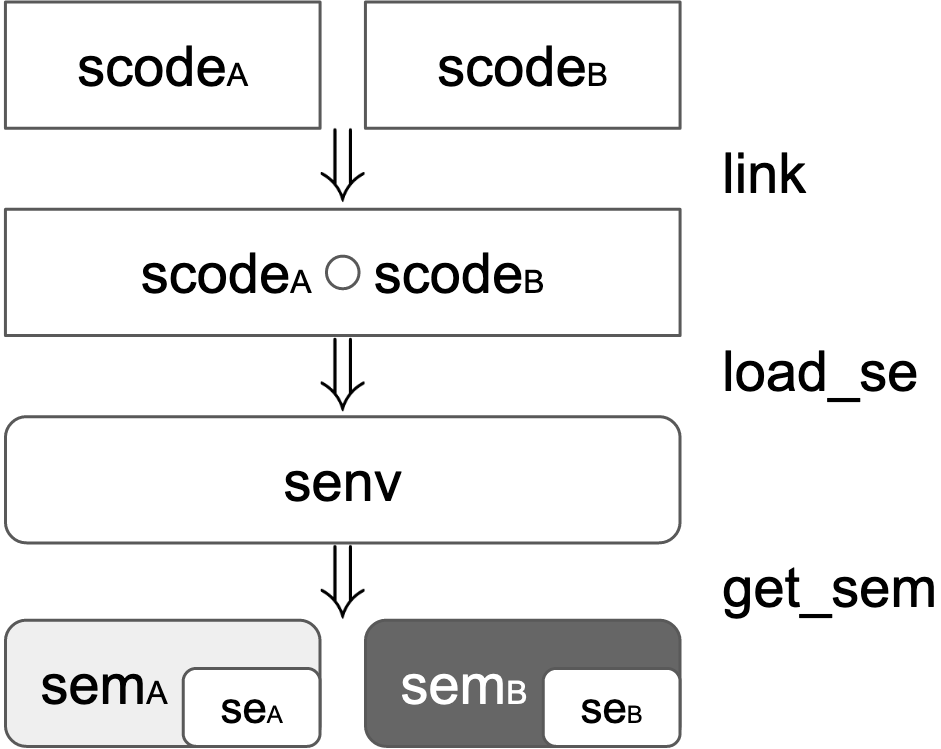
\includegraphics[width=1\linewidth]{fig-load.png}
%% \caption{Loading Process}
%% \label{fig:load}

%% \begin{minipage}{0.5\linewidth}
%% \begin{figure}
%%   \centering
%%   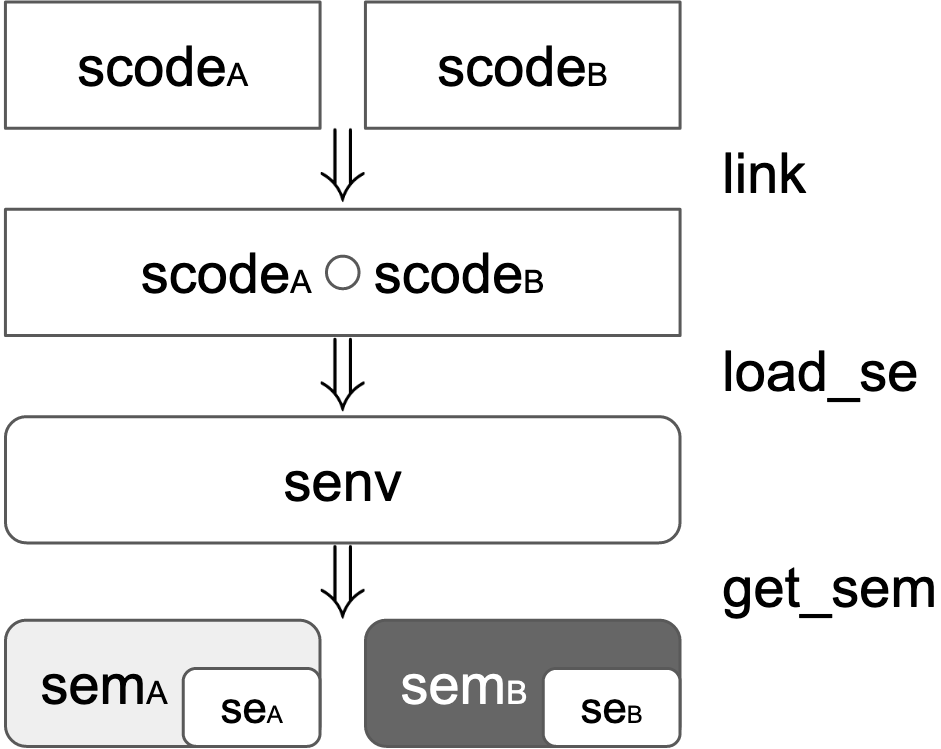
\includegraphics[width=0.25\linewidth]{fig-load.png}
%%   \caption{Loading Process}
%%   \label{fig:load}
%% \end{figure}
%% \end{minipage}

%% \begin{subfigure}{.4\linewidth}
%%   \centering
%%   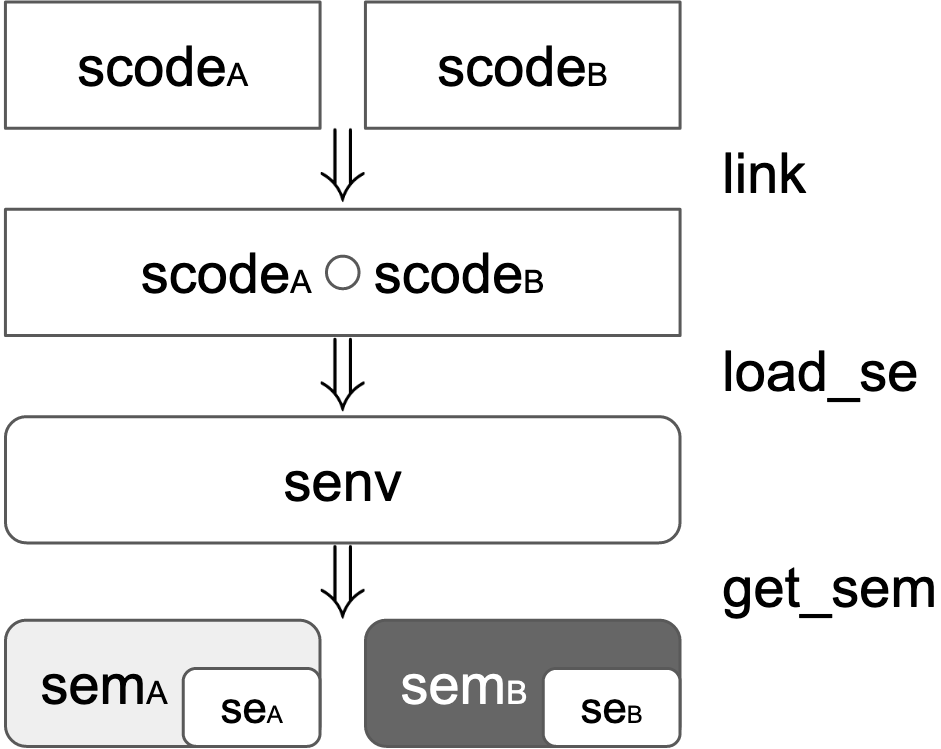
\includegraphics[width=0.25\linewidth]{fig-load.png}
%%   \caption{Loading Process}
%%   \label{fig:load}
%% \end{subfigure}

%% \youngju{lookup\_modsem is actually deterministic (loading process guarantees it)}

%% \youngju{Maybe we can use ``bar'' notation like princeton did}
\caption{Loading in Interaction Semantics}
\label{fig:full-sem}
\vspace*{-2mm}
\end{wrapfigure}



Loading the initial states of multiple modules requires an interesting
coordination of the modules, especially in the presence of module-local static variables.  In essence, we
should disallow accesses to a static variable from other modules than the defining one.  For
this, the loading of modules $M_1, \cdots, M_n$ proceeds as follows, which is illustrated for two
modules in \Cref{fig:full-sem}.

First, each module has \emph{symbol code}, which consists of symbols (\ie global variables and functions) and their
signatures (\eg{} \code{x: int}, \code{f: void(int)}).  For each $i$, let $M_i.\code{scode}$ be the
symbol code of $M_i$.  Crucially, symbol codes have the same type even if their modules are written
in different languages.

Second, since symbol codes have the same type, we can calculate the physical linking
$sc = M_1.\code{scode} \plink \cdots \plink M_n.\code{scode}$ of the symbol codes of modules.  Now
$sc$ is the symbol code for entire program consisting of all the symbols and signatures.  The
physical linking is defined in \cite{kang:scc}.

Third, we load $sc$ to get the initial memory $mem$ \newnewrevision{(by \textrm{load\_mem})}
and the program's global \emph{symbol environment}~$se$ \newnewrevision{(by \textrm{load\_se})},
which is the run-time information of symbols (\eg{} \code{x} points to
\code{0x700} and \code{f} points to \code{0x800}).  This loading process follows the original \cc{}'s.

Fourth, we initialize module semantics for each module $M_i$ with the program's global symbol
environment $se$.  In particular, we calculate $M_i$'s local environment, which contains information
of \emph{only} those symbols defined in the module.  Crucially, this prevents the other modules from
accessing the static variables of $M_i$. Note that \ccc{} does not have local environments because it does not support static variables.

Finally, the initial memory and module semantics form the initial state for interaction semantics.

%% Here, it is crucial to distinguish global and local environments for controlling accesses to
%% static variables.  Note that 

% restriction phase didn't exist in \ccc{}: instead, all the symbols were put in each module's
% symbol environment.  At that time there was no static variable, so it was fine, but now we have to
% (at least) remove other module's static variables, and we chose the most cannonical way (low
% cognitive overhead).



% Each \cc{}'s program is of type $program \; F \; V$ (static info) where F and V differs for each
% language.  F stands for function definition and V stands for info on variable definition
% (e.g. type).  Each \cc{}'s global environment (runtime info) is of type $Genv \; F \; V$.  In global
% environment, each symbol is mapped to some block in \Memory.

% communications between modules, while \ccc{} only supported C-style. Currently, Asm-style
% communication is only allowed between Asm modules (this is the same for \ccx{}.

% \youngju{FYI: bottom left of page 5 of \ccc{}'s paper explains the same thing}

% $\Skel \defeq program \; \option{sig} \; unit$ \hspace{4mm} and \hspace{4mm}
% $\Skenv \defeq Genv \; \option{sig} \; unit$ \hspace{4mm} where \hspace{4mm}
% $ \option{a} \defeq a \uplus \emptyset $.
%% \youngju{iris notation} 

% Loading process figure: square box is static info, and rounded box is runtime info. Grey ones are
% language-specific ones, and white ones are language-agnostic ones.

% Loading process should (i) give a compatible view on symbol-memory mapping, and (ii) initialize
% global variable's corresponding memory (iii) gives failure when static variable is declared in
% another module.  To this end, we use standard, off-the-shelf \cc{} linker and loader (linker is
% very slightly modified).  The linker takes uni-language modules so we first extract
% language-agnostic part of each program and to make it uni-language.  Then, we link and load it to
% get ``big'' symbol environment.  Finally, each module uses this ``big'' one to initialize its
% module semantics, resulting in ``small'' symbol environments for each one.  The ``small'' ones are
% restricted from big ones so that only symbols declared in its code are visible.  Note that, such
% restriction phase didn't exist in \ccc{}: instead, all the symbols were put in each module's
% symbol environment.  At that time there was no static variable, so it was fine, but now we have to
% (at least) remove other module's static variables, and we chose the most cannonical way (low
% cognitive overhead).

% It is not explicit in the figure, but $\texttt{load\_mem}(\texttt{A.c} \circ \texttt{B.c})$ will be
% used as an initial memory of interaction semantics.

%% \youngju{We don't need to mention (i) $\plink$ is the one introduced in \cite{TODO} and (ii) it is for single language}
% Interaction semantics is trivial, so we skip it.


% \youngju{In opensim, there are also some difference with presentation and Coq but they are
% equivalent.}

%% Note that in our overview's presentation, the language state and memory were separated.
%% But in our formalization, we chose not to: \cc{} does not separate language state and memory, and we want to reduce diff from \cc{}.
%% As a consequence, our CallData/Retdata contains memory, conveying ``current'' memory.
%% Both representations (separated or not) are equivalent.


%% \youngju{we separated memory and state in main:verification. Then, we need to separate here too}

%% \youngju{IMPORTANT: We omitted system module. However, we required $\SREL{}$ -(7) for system module, so this condition is orphaned now.}




\subsection{Module Semantics}
\label{sec:main-semantics:module}

%% We briefly discuss differences between the module semantics of \ccm{} presented in
%% \Cref{fig:modsem} and that of \ccc{} described in \Cref{sec:overview-semantics:background}.
%% Our module is different from that of \ccc{} on loading.

We briefly discuss the notions of module and module semantics presented in \Cref{fig:modsem}.
%
To support loading described in \Cref{sec:main-semantics:loading},
a module $M$ consists of $M\code{.scode}$, which is its symbol
code, and $M\code{.get\_sem}$, which returns a module semantics given a program's symbol environment.
The local environment \code{senv} of the module semantics should coincide with the
global environment restricted on $M\code{.scode}$.

%% The module semantics is almost the same with the presentation in the \Cref{sec:overview-semantics:background}.
%% \begin{itemize}
%% \item $\code{senv}$: A symbol environment that determines if a symbol belongs to the module semantics.
%% \item \code{init\_core}: constructs an initial machine state from the given call data, where call data is a triple representing current memory, function pointer, and its arguments. We purposely defined this operation as a predicate rather than a function in order to address nondeterminism introduced in \Cref{sec:overview-semantics:solution}.
%% \item \code{at\_external}: given a machine state, returns call data if the machine state is calling an external function, and nothing otherwise.
%% \item \code{halted}: given a machine state, returns return data (a pair representing current memory and return value) if the machine state is returning, and nothing otherwise. 
%% \item \code{after\_external}: given a machines state and return data, updates the machines state accordingly.
%% \end{itemize}

%% Few things to note here are as follows:
%% We support not only C-style but also assembly-style call and return data passing for assembly functions that does not comply with the C calling convention.
%% Assembly-style call data and return data are composed of a memory and a register file. Like \ccx{}, only assembly
%%   modules are allowed to perform assembly-style calls.

The module semantics of \ccm{} is slightly more general than that presented in \Cref{sec:compiler:background}.
\begin{itemize}
\item A module semantics has a symbol environment $\code{senv}$ that determines whether a symbol belongs to the module or not.
\item \code{init\_core} is defined as a predicate rather than a function in order to allow such nondeterminism introduced in \Cref{sec:compiler:solution}.
\item Module operations other than \code{corestep} (denoted here $\estep{}$) can also change the
  memory, which is needed to turn on and off the access permission of the arguments area as discussed in \Cref{sec:compiler:solution}.
  %% Thanks to such flexibility, our \code{corestep} relation remains unchanged from the language steps in \cc{}.
\item Module semantics supports not only C-style but also assembly-style calling convention in the sense of \ccx{},
  where the former just passes argument and return values between the caller and callee while the latter the whole register file.
  %% which passes the whole register file information between the caller and callee instead of just argument and return values.
  %% for assembly functions that does not comply with the C calling convention.
  %% Assembly-style call and return data are composed of a memory and a register file.
  Like \ccx{}, only assembly functions are allowed to make assembly-style calls.
\end{itemize}

%% Our module semantics is different from that of \ccc{} in the following ways:
%% \begin{itemize}
%% \item A module semantics has a symbol environment $\code{senv}$ that determines if a
%%   symbol belongs to the module semantics or not.
%% \item \code{init\_core} is a predicate rather than a function to take into account nondeterminism.
%% \item Not only \code{corestep} but also all the others change memory, for the purpose of identifying
%%   core steps with the language steps in \cc{}.\footnote{Also for the purpose of identifying core
%%     steps with the language steps in \cc{}, unlike the presentation here, our Coq formalization
%%     actually does not explicitly split a machine state into a memory and a module state.}  Memory
%%   accesses introduced in interaction semantics, such as preparation for outgoing arguments area, are
%%   now performed in \eg{} \code{init\_core}.
%%   % 스텝말고 나머지도 메모리 변경.  core step = underlying step.  init\_core, ... 등에서 marshalling
%%   % 등 처리
%% \item Module semantics supports not only C-style but also assembly-style call and return value
%%   passing.  At call sites, \code{at\_external} checks if the given machine state is about to invoke
%%   an external call with a call data of type \textrm{CallData}.  A call data is either $(i)$ C-style,
%%   consisting of a memory, a function pointer, and argument values, or $(ii)$ assembly-style,
%%   consisting of a memory, a function pointer, and a register file.  On the other hand, on return,
%%   \code{after\_external} is given a return data of type \textrm{ReturnData}, and produces the next
%%   state.  A return data is also either $(i)$ C-style, consisting of a memory and a return value, or
%%   $(ii)$ assembly-style, consisting of a memory and a register file.  Like \ccx{}, only assembly
%%   modules are allowed to perform assembly-style calls.
%% \end{itemize}

\begin{figure}[t!]
\footnotesize

%% trick from: https://tex.stackexchange.com/questions/391318/make-figure-with-minipages-wider-than-text
\makebox[\linewidth]{\makebox[1.2\linewidth]{
\begin{minipage}{1.2\linewidth}
  \mytitle{module}\\
$
  \begin{stackTL}
  \begin{array}{l@{}l}
  \module \in \Module = \{ & (\texttt{scode}, \texttt{get\_sem}) \in (\Skel \times (\Skenv \rightarrow \Msem)) \; | \; \forall \skenv, \texttt{get\_sem}(\skenv).\texttt{senv} = \skenv \textbar_{\texttt{scode}}
                        \} \\
  \end{array}
  \end{stackTL}
$
\end{minipage}%
}}
\\
\makebox[\linewidth]{\makebox[1.2\linewidth]{
\begin{minipage}{1.2\linewidth}
  \mytitle{module semantics}\\
$
  \begin{stackTL}
  \begin{array}{@{}l@{}}
    \msem \in \Msem = \\
    \quad  \setof{ \myst \in \textrm{Set}, \texttt{senv} \in \Skenv, \estep{} \; \in \powset{(\Memory \times \myst) \times \Events \times (\Memory \times \myst)}, \\
    \quad\ \ \;\texttt{init\_core} \in \Args \rightarrow \powset{\Memory \times \myst}, \\
    \quad\ \ \;\texttt{at\_external} \in (\Memory \times \myst) \rightarrow \option{\Args}, \\
    \quad\ \ \;\texttt{after\_external} \in (\myst \times \Retv) \rightarrow \option{(\Memory \times \myst)}, \\
    \quad\ \ \;\texttt{halted} \in (\Memory \times \myst) \rightarrow \option{\Retv} \; | \\
    \quad\ \ \;\{ \ms \;|\; \exists e, \ms',~ \ms \estep{e} \ms' \}, \{ \ms \;|\; \exists \args, \texttt{at\_external}(\ms) = \some{\args} \},
               \{ \ms \;|\; \exists \retv, \texttt{halted}(\ms) = \some{\retv} \} \text{ disjoint}
    } \\
  \end{array}
  \\
  \begin{array}{l@{}l@{}l}
    \Args & \defeq \{ (\texttt{m}, \texttt{f}, \texttt{vs}) \in (\Memory \times \Val \times \overrightarrow{\Val}) \} & \; \uplus \;
                   \{ (\texttt{m}, \texttt{f}, \texttt{rs}) \in (\Memory \times \Val \times (\Reg \rightarrow \Val)) \} \\
    \Retv & \defeq \{ (\texttt{m}, \texttt{v}) \in (\Memory \times \Val) \} & \; \uplus \;
                   \{ (\texttt{m}, \texttt{rs}) \in (\Memory \times (\Reg \rightarrow \Val)) \} \\
    %% \args.\texttt{f} & \defeq \textbf{match} \; \args \; \textbf{with}~~
    %%                    \mathtt{|}~ \textbf{left}~ \args \Rightarrow \args.\texttt{f}~
    %%                    \mathtt{|}~ \textbf{right}~ \args \Rightarrow \args.\texttt{rs}(\textbf{PC})~
    %%                    \textbf{end} \span \\
  \end{array}
  \end{stackTL}
$
\\
\end{minipage}
}}

%% \youngju{Use [ $\defeq$ ] for [ $\module \in \Module =$ ]? If so, we should change this fig and fig-param too.}

\caption{Module and Module Semantics \vspace{5mm} \mbox{}}
\label{fig:modsem}
\end{figure}


\section{Formalization of Verification Techniques}
\label{sec:compiler:verification}

Now we present the formalization of our verification techniques.
%% As discussed in \Cref{sec:overview-verification:solution},
We parameterize the notion of open simulation presented in
\Cref{sec:overview-verification} with three parameters: memory relations, symbol
relations, and memory predicates.  We present the three parameters
(\Cref{sec:main-verification:parameter}), the parameterized open simulations
(\Cref{sec:main-verification:opensim}), and their horizontal compositionality and adequacy theorems
(\Cref{sec:main-verification:theorems}).
%% Then we introduce mixed simulation that allows forward
%% reasoning in the presence of nondeterminism (\Cref{sec:main-verification:mixedsim}).

\subsection{Parameters for Open Simulations}
\label{sec:main-verification:parameter}

\Cref{fig:simulation-parameters} presents
the sets of three parameters for open simulations:
the set of memory relations $\MREL$, the set of symbol relations $\SREL$, and the set of memory predicates $\MPRED$.
%% , which we will explain in details.
%% Note that this section will be easier to follow if read in color:
%% \textcolor{myred}{memory relations} are presented in red, \textcolor{darkgreen}{symbol relations} in
%% green, and \textcolor{myblue}{memory predicates} in blue.

\begin{figure}[t!]
\footnotesize

\makebox[\linewidth]{\makebox[1.2\linewidth]{
\begin{minipage}{1.2\linewidth}
  \vspace{3mm}\mbox{}\\
  \mytitle{memory relation}\\
$
  %% \[
  \begin{stackTL}
  %% \MREL = \{
  %% (\ty, \texttt{mem}, \sqsubseteq, \sqsubseteq_\pub, \texttt{vrel}) \; | \;
  %% \ty \in \textrm{Set}, \texttt{mem} \in \ty \rightarrow (\Memory \times \Memory), \sqsubseteq, \sqsubseteq_\pub \; \in \powset{\ty \times \ty}, \texttt{vrel} \in \ty \rightarrow \powset{\Val \times \Val}
  %% %% & \ty \in \textrm{Set}, \texttt{src} \in \ty \rightarrow \Memory, \texttt{tgt} \in \ty \rightarrow \Memory, \sqsubseteq, \sqsubseteq_\pub \; \in \powset{\ty \times \ty}, \texttt{vrel} \in \ty \rightarrow \powset{\Val \times \Val}
  %% \}
  %% \\
  %% \MREL \text{ is a \emph{MemRel} if the following properties hold.}
  %% \\
  %% \\
  %% \caselabel{properties}\\
  %% {\begin{array}{l@{\;}l}
  %%   \caselabel{1} & \sqsubseteq_\pub \text{ is preorder}\\
  %%   \caselabel{2} & \sqsubseteq_\pub \subseteq \sqsubseteq\\
  %%   \caselabel{3} & \forall \mrel, \mrel',\; \mrel \sqsubseteq \mrel' \implies \texttt{vrel}(\mrel) \subseteq \texttt{vrel}(\mrel')\\
  %% \end{array}}
  %% \\
  %% %% \texttt{mrel}: \ty \rightarrow \powset{\Memory \times \Memory} \defeq \lambda \mrel, \mem_\src, \mem_\tgt, ($\MREL{}$.\texttt{src} \; \mrel) = \mem_\src \land ($\MREL{}$.\texttt{tgt} \; \mrel) = \mem_\tgt \\
  %% \caselabel{derived}\\
  %% \begin{array}{r@{\;}l}
  %% \texttt{mrel} & \defeq \lambda \mrel, \mem_\src, \mem_\tgt,\; ($\MREL{}$.\texttt{src} \; \mrel) = \mem_\src \land ($\MREL{}$.\texttt{tgt} \; \mrel) = \mem_\tgt \\
  %% \args_\src \succsim_{\mrel} \args_\tgt & \defeq (\args_\src.\texttt{f}, \args_\tgt.\texttt{f}) \in \texttt{vrel}(\mrel) \land
  %%   (\args_\src.\texttt{mem}, \args_\tgt.\textrm{mem}) \in \texttt{mrel}(\mrel) \land
  %%   (\args_\src.\texttt{vs}, \args_\tgt.\texttt{vs}) \in \overrightarrow{\texttt{vrel}(\mrel)}\\
  %% \retv_\src \succsim_{\mrel} \retv_\tgt & \defeq (\retv_\src.\texttt{v}, \retv_\tgt.\texttt{v}) \in \texttt{vrel}(\mrel) \land
  %%   (\retv_\src.\texttt{mem}, \retv_\tgt.\textrm{mem}) \in \texttt{mrel}(\mrel)\\
  %% \end{array}
  %% \\
  %% .
  %% \\
  %% .
  %% \\
  %% .
  %% \\


  \begin{array}{l@{}l}
  \MREL \in \textrm{MemRel} = \span
  \\\quad
  \setof{
    (&\ty, \sqsubseteq, \sqsubseteq_\weak, \texttt{mrel}, \texttt{vrel}) \in (\textrm{Set} \times \powset{\ty \times \ty} \times \powset{\ty \times \ty} \times (\ty \rightarrow \powset{\Memory \times \Memory}) \times (\ty \rightarrow \powset{\Val \times \Val})) \; |
  \\\quad
  & (\sqsubseteq \text{ is preorder}) \; \land \;
    (\sqsubseteq \, \subseteq \, \sqsubseteq_\weak) \; \land \;
    (\forall \mrel, \mrel',\; \mrel \sqsubseteq \mrel' \implies \texttt{vrel}(\mrel) \subseteq \texttt{vrel}(\mrel')) \; \land \;
  \\\quad
  & (\forall \mrel, i,~ (\textrm{Vint } i, v_\tgt) \in \texttt{vrel}(\mrel) \implies v_\tgt = \textrm{Vint } i)
  }
  \end{array}
  \\
  %% \texttt{mrel}: \ty \rightarrow \powset{\Memory \times \Memory} \defeq \lambda \mrel, \mem_\src, \mem_\tgt, ($\MREL{}$.\texttt{src} \; \mrel) = \mem_\src \land ($\MREL{}$.\texttt{tgt} \; \mrel) = \mem_\tgt \\
  \begin{array}{r@{\;}l}
  \args_\src \succsim_{\mrel} \args_\tgt \defeq &
    (\args_\src.\texttt{m}, \args_\tgt.\texttt{m}) \in \texttt{mrel}(\mrel) \land
    (\args_\src.\texttt{f}, \args_\tgt.\texttt{f}) \in \texttt{vrel}(\mrel) \land
    (\args_\src.\texttt{vs}, \args_\tgt.\texttt{vs}) \in \overrightarrow{\texttt{vrel}(\mrel)} \; \land \\
    & (\args_\src.\texttt{rs}, \args_\tgt.\texttt{rs}) \in \overrightarrow{\texttt{vrel}(\mrel)} \\
  \retv_\src \succsim_{\mrel} \retv_\tgt \defeq &
    (\retv_\src.\texttt{m}, \retv_\tgt.\texttt{m}) \in \texttt{mrel}(\mrel) \land
    (\retv_\src.\texttt{v}, \retv_\tgt.\texttt{v}) \in \texttt{vrel}(\mrel) \land
    (\retv_\src.\texttt{rs}, \retv_\tgt.\texttt{rs}) \in \overrightarrow{\texttt{vrel}(\mrel)} \\
  \end{array}
  \end{stackTL}
$
  %% \]
%% \youngju{\texttt{vrel} should be $\MREL{}$.\texttt{vrel}. (1) change? note that Former (and overview) is textrm but latter is texttt (2) specify $\MREL{}$ only when it is confusing (e.g. \ty)}
\\
\end{minipage}%
}}
\\
\makebox[\linewidth]{\makebox[1.2\linewidth]{
\begin{minipage}{1.2\linewidth}
  \vspace{3mm}\mbox{}\\
  \mytitle{symbol relation}\\
$
  \begin{stackTL}
  \begin{array}{@{}l@{}l@{~}l@{}}
    \SREL \in \textrm{SymbRel} = \span \span
\\\quad
\setof{&(\ty, \sqsubseteq, \simsk, \simskenv) \in
(\textrm{Set} \times \powset{\ty \times \ty} \times (\ty \rightarrow \powset{\Skel \times \Skel}) \times (\ty \rightarrow \MREL.\ty \rightarrow \powset{\Skenv \times \Skenv})) \; | \span
\\\quad
& \caselabel{1} \;&  \sqsubseteq \textrm{is preorder}
\\\quad
& \caselabel{2} \;& \forall \skel_\src, \skel'_\src, \skel''_\src, \skel_\tgt, \skel'_\tgt, \skel''_\tgt,~ \skel''_\src = \skel_\src \plink \skel'_\src \land \skel''_\tgt = \skel_\tgt \plink \skel'_\tgt \implies {}
\\\quad
&                   &
\forall \srel, \srel',~ (\skel_\src, \skel_\tgt) \in \simsk(\srel) \land (\skel'_\src \; \skel'_\tgt) \in \simsk(\srel') \implies {}
\\\quad
&                   &
\exists \srel'',~ (\skel''_\src, \skel''_\tgt) \in \simsk(\srel'') \land \srel \sqsubseteq \srel'' \land \srel' \sqsubseteq \srel''
\\\quad
& \caselabel{3} \; & \forall \skel_\src, \skel_\tgt, \srel,~ (\skel_\src, \skel_\tgt) \in \simsk(\srel) \implies
\\\quad
  &                   & \exists \mrel,~ (\textrm{load\_mem}(\skel_\src), \textrm{load\_mem}(\skel_\tgt)) \in \texttt{mrel}(w) \; \land \;
(\textrm{load\_se}(\skel_\src), \textrm{load\_se}(\skel_\tgt)) \in \simskenv(\srel, \mrel)
\\\quad
& \caselabel{4} \; & \forall \srel, \mrel, \mrel',~ \mrel \sqsubseteq_\weak \mrel' \implies \simskenv(\srel, \mrel) \subseteq \simskenv(\srel, \mrel')
\\\quad
  %% & \caselabel{5} \; (& \forall \srel, \mrel, \skenv_\src, \skenv_\tgt, \val_\src, \val_\tgt,~ (\skenv_\src, \skenv_\tgt) \in \simskenv(\srel, \mrel) \land (\val_\src, \val_\tgt) \in \MREL.\texttt{vrel}(\mrel) \implies \\
  %% &                   & \val_\src \in \textrm{ftns}(\skenv_\src) \iff \val_\tgt \in \textrm{ftns}(\skenv_\tgt))\\
& \caselabel{5} \; & \forall \srel, \mrel, \skenv_\src, \skenv_\tgt,~ (\skenv_\src, \skenv_\tgt) \in \simskenv(\srel, \mrel) \implies \skenv_\src.\texttt{pubs} = \skenv_\tgt.\texttt{pubs} \; \land \;
\\\quad
&                   & \forall (v_\src, v_\tgt) \in \MREL.\texttt{vrel}(\mrel),~ v_\src \in \textrm{ftns}(\skenv_\src) \implies v_\tgt \in \textrm{ftns}(\skenv_\tgt)
\\\quad
& \caselabel{6} \; & \forall \srel, \srel', \mrel, \skel_\src, \skel_\tgt, \skenv_\src, \skenv_\tgt,~

                     \srel \sqsubseteq \srel' \land (\skel_\src, \skel_\tgt) \in \simsk(\srel) \land (\skenv_\src, \skenv_\tgt) \in \simskenv(\srel', \mrel) \implies
\\\quad
&                   & (\skenv_\src \textbar_{\skel_\src}, \skenv_\tgt \textbar_{\skel_\tgt}) \in \simskenv(\srel, \mrel)
\\\quad
& \caselabel{7} \; & \forall \srel, \mrel, \skenv_\src, \skenv_\tgt, \args_\src, \args_\tgt,~ (\skenv_\src, \skenv_\tgt) \in \simskenv(\srel, \mrel) \land \args_\src \succsim_{\mrel{}} \args_\tgt \implies
\\\quad
  &                   & \forall e, \retv_\src,~ \textrm{external\_call} \; \skenv_\src \; \args_\src \; e \; \retv_\src \implies \exists \retv_\tgt,~ \textrm{external\_call} \; \skenv_\tgt \; \args_\tgt \; e \; \retv_\tgt \land
                        \exists \mrel' \sqsupseteq \mrel,~ \retv_\src \succsim_{\mrel'} \retv_\tgt
  }
  \end{array}
  \\
  \end{stackTL}
$
\end{minipage}%
}}
\\
\makebox[\linewidth]{\makebox[1.2\linewidth]{
\begin{minipage}{1.2\linewidth}
  \vspace{3mm}\mbox{}\\
  \mytitle{memory predicate}\\
$
  \begin{stackTL}
  \begin{array}{l@{}l}
  \MPRED \in \textrm{MemPred} = \span \\
  \quad \setof{ (&\ty, \sqsubseteq, \sqsubseteq_\weak, \texttt{mpred}, \texttt{vpred}, \texttt{sepred}) \in (\textrm{Set} \times \powset{\ty \times \ty} \times \powset{\ty \times \ty}
                                                                                                           \times (\ty \!\rightarrow\! \powset{\Memory}) 
                                                                                                           \times (\ty \!\rightarrow\! \powset{\Val}) \times (\ty \!\rightarrow\! \powset{\Skenv})) \; | \\
  & (\sqsubseteq \text{ is preorder}) \; \land \;
  (\sqsubseteq \, \subseteq \, \sqsubseteq_\weak) \; \land \;
  (\forall \mpred, \mpred',\; \mpred \sqsubseteq \mpred' \implies \texttt{vpred}(\mpred) \subseteq \texttt{vpred}(\mpred')) \; \land \; \\
  & (\text{\texttt{sepred} should satisfy the unary version of $\simskenv$'s conditions where $\SREL{}.\!\!\sqsubseteq$ and $\simsk$ are the total relations})
  }
  \end{array}
  \\
  \begin{array}{r@{\;}l}
  %% \texttt{mpred}(\mpred) & \defeq \setof{$\MPRED{}$.\texttt{mem}(\mpred)} \\

  \texttt{cpred}(\mpred) & \defeq \{ \args \in \Args \suchthat \args.\texttt{m} \in \texttt{mpred}(\mpred) \land \args.\texttt{f} \in \texttt{vpred}(\mpred) \land
                                                \args.\texttt{vs} \in \overrightarrow{\texttt{vpred}(\mpred)} \land \args.\texttt{rs} \in \overrightarrow{\texttt{vpred}(\mpred)} \} \\
  \texttt{rpred}(\mpred) & \defeq \{ \retv \in \Retv \suchthat \retv.\texttt{m} \in \texttt{mpred}(\mpred) \land \retv.\texttt{v} \in \texttt{vpred}(\mpred) \land
                                                \retv.\texttt{rs} \in \overrightarrow{\texttt{vpred}(\mpred)} \} \\
  %% \args_\src \in \texttt{cpred}(\mpred) & \defeq \args_\src.\texttt{m} \in \texttt{mpred}(\mpred) \land \args_\src.\texttt{f} \in \texttt{vpred}(\mpred) \land
  %%                                               \args_\src.\texttt{vs} \in \overrightarrow{\texttt{vpred}(\mpred)} \land \args_\src.\texttt{rs} \in \overrightarrow{\texttt{vpred}(\mpred)} \\
  %% \retv_\src \in \texttt{rpred}(\mpred) & \defeq \retv_\src.\texttt{m} \in \texttt{mpred}(\mpred) \land \retv_\src.\texttt{v} \in \texttt{vpred}(\mpred) \land
  %%                                               \retv_\src.\texttt{rs} \in \overrightarrow{\texttt{vpred}(\mpred)} \\

  \end{array}
  \end{stackTL}
$
%% \\
%% \youngju{지금 2번쨰줄 아래가 짤리는데 왜인지 모르겠습니다}\\
%% \youngju{pred 대신 prd?}\\
\end{minipage}
}}

\caption{Three parameters for open simulations}
\label{fig:simulation-parameters}
\end{figure}


\myparagraph{Memory Relation}

The first parameter ranges over Kripke-style memory/value relations in $\MREL$.
%~\cite{DBLP:conf/popl/AhmedDR09}
Following \cite{DBLP:conf/icfp/DreyerNB10,pb}, we model the
evolution of memory relations using \emph{possible worlds} and \emph{private and public transitions}
over the worlds.
Note that this parameter will be instantiated with the three memory relations used in \cc{}---namely memory
identity, extension, and injection---and the memory injection with module-local invariants we introduced.
%% for verifying \texttt{Unreadglob}.

A memory relation in $\MREL$ consists of $(i)$ a set $\code{t}$ of possible worlds; $(ii)$ \emph{public}
and \emph{private} transition relations $\sqsubseteq$ and $\sqsubseteq_\weak$ over the worlds;
and $(iii)$ for each world $w \in \code{t}$, memory relation $\texttt{mrel}(w)$ and
value relation $\texttt{vrel}(w)$.  A world $w$ represents an invariant on the memory, which
can evolve over time according to the public/private transition relations,
as we discussed in \Cref{sec:overview-verification:injection}.
%% public transitions $\sqsubseteq$ represent possible evolution of the world before and after an external function
%% call, and private transitions $\sqsubseteq_\weak$ represent possible evolution between any two interaction points with
%% external modules. %(\eg{} between two invocations of external functions).
%% For example, we use private transitions to capture the permission changes in the arguments area of the stack,
%% which cannot be public transitions according to the \newnewrevision{enriched} memory injection.
%% For example, memory
%% injection's public transition encodes the invariant that injection should be increased and memory
%% access permissions are the same before and after a function call; but its private transition allows
%% certain changes in access permissions, as discussed in \Cref{sec:overview-semantics:solution}.  The
%% public transition relation is reflexive and transitive, and is a subset of the private transition
%% relation.
There are four natural well-formedness conditions, which are self-explanatory.
%% $\texttt{vrel}(w)$ should be monotone w.r.t. the world's private
%% transition, and it relates an integer value in source only with the same value in target.
We can also straightforwardly extend the value/memory relation to relations on $\Args$ and $\Retv$, denoted $\succsim_{\mrel}$.
%% For each
%% world $w \in \code{t}$, relations on the input/output of external function calls are defined in a
%% straightforward manner: function pointers, arguments, and results are related as values, and
%% input/output memories are related as memories.

\myparagraph{Symbol Relation}

The second parameter ranges over symbol relations in $\SREL$ that
relate information about global symbols (\eg which block each global
variable points to) in the source and target.  This parameter is
needed to verify optimizations like \code{Unusedglob},
\code{Unreadglob} that remove unnecessary static variables thereby
having non-identical symbol information in the source and target.

%% enables he verification of such
%% specifications and optimizations as \code{Unusedglob} that change symbol tables.
%% Verification of
%% all \cc{} optimizations, except for \code{unused-globs}, requires only a trivial symbol relation
%% in which the source and target symbols are exactly the same.  The main purpose of $\SREL$ is
%% guaranteeing a \emph{run-time} symbol relation, assuming all its modules satisfy \emph{compile-time}
%% symbol relation.  We allow modular reasoning of symbol relations using states and their
%% compatibility relation w.r.t. linking.  For example, the verification of \code{unused-globs} uses a
%% symbol relation whose state is the set of dropped symbols.  To model the evolution of symbol
%% relations under linking, we say two states are compatible if the former is a subset of the latter.
%% The compile-time and run-time symbol relations check whether the symbols in the state are actually
%% dropped.
%% Specifically,

A symbol relation in $\SREL$ consists of $(i)$ a set $\code{t}$ of symbol relation states; $(ii)$ 
an extension relation $\sqsubseteq$ on the states; $(iii)$ for each state $d$,
a (compile-time) symbol code relation $\texttt{screl}(d)$; and $(iv)$ for each state $d$ and world $w \in \MREL.\code{t}$,
(run-time) symbol environment relation $\texttt{serel}(d,w)$.
There are seven well-formedness conditions:
%% $\SREL$ should satisfy the following conditions:
$(1)$ the extension relation $\sqsubseteq$ is transitive and reflexive;
$(2)$ \texttt{screl} is closed under the syntactic linking;
$(3)$ if symbol codes are related by \texttt{screl}, then \newnewrevision{the initial memories and symbol environments loaded by \textrm{load\_mem} and \textrm{load\_se} are related by \texttt{mrel} and \texttt{serel}, respectively};
$(4)$ \texttt{serel} is monotone w.r.t. private transitions;
$(5)$ \newnewrevision{for symbol environments related by \texttt{serel}, their public symbols are identical and their functions have the same signatures};
$(6)$ \texttt{serel} is compatible with $\sqsubseteq$: for $d \sqsubseteq d'$, $\texttt{serel}(d')$ restricted on $\texttt{screl}(d)$ should be in $\texttt{serel}(d)$; and
%% is preserved w.r.t. compatible restriction on symbol codes; and
$(7)$ the memory and symbol relations should be compatible with \cc{}'s axiom about system calls (\ie \textrm{external\_call}).
%% external function symbols related by \texttt{serel} satisfy the condition for open simulation.

% \cdashbox{darkgreen}{$\texttt{screl}(d)$} statically holds for some $d \sqsubseteq d'$ at compile time.



% (0) \SREL{}는 크게 3가지로 instantiate 된다: identity, drop (unusedglob용), invariant (spec 증명용).
%    t 는 두 symbol code (lanugage-dependent 한 부분을 걷어낸 코드)를 relate (screl) 하는데 쓰인다.
%    identity의 경우 unit 타입이고 screl은 항상 true이다.
%    drop의 경우 set of symbol이고 screl은 (i) 실제로 그 symbol이 빠졌는지 (ii) 그 symbol을 refer하는게 없는지 체크한다. (injection 매핑에서 빼줘야 하기 때문)
%    invariant의 경우 역시 set of symbol이고 screl은 (i) 실제로 그 symbol이 invariant를 만족하는지 (ii) 그 symbol을 refer하는게 없는지 체크한다. (injection 매핑에서 빼줘야 하기 때문)
%    $\sqsubseteq$의 의미는 대충 set inclusion 이다. \\
%    이 interface의 모든 목적은 static하게 $\cfbox{darkgreen}{screl}$ 을 guarantee 해주면 runtime에 $\cdashbox{darkgreen}{serel}$ 를 rely 받는 것이다. \\

% (5) serel이면 (i) public symbol들이 같고 (ii) 어떤 relate되어있는 src/tgt value가 있을 때, src가 function이면 tgt도 function이고 둘의 signature가 같다. \\
% (6) 큰 senv가 큰 d'에 대해 serel이고, 작은 sc가 작은 d에 대해 screl이면, 각각의 큰 senv를 작은 sc로 restrict 한 것도 relate 되어있다. \\
% (7) external call axiom \\



\myparagraph{Memory Predicate}

The third parameter ranges over Kripke-style memory predicates in $\MPRED$,
which are needed to modularly verify \cc{}'s analysis engines such as value analysis (see \Cref{sec:main-verification:opensim}).
%% based on which is proved the soundness of compiler's analyses such as \cc{}'s value analysis.
$\MPRED$ is essentially a unary version of $\MREL$ combined with $\SREL$
where $\SREL{}.{\sqsubseteq}$ and $\simsk$ are taken as the total relations (\ie relating everything):
it consists of
$(i)$ the set $\code{t}$ of possible worlds;
$(ii)$ public and private transition relations $\sqsubseteq$ and $\sqsubseteq_\weak$ over the worlds, respectively; and
$(iii)$ for each world $w \in \code{t}$, a memory predicate $\textrm{mpred}(w)$,
a value predicate $\textrm{vpred}(w)$, and a symbol environment predicate $\textrm{sepred}(w)$.
The well-formedness conditions are self-explanatory.
%% Similarly to $\MREL$, $(i)$ $\MPRED$ has world's public and private transitions; $(ii)$ its value
%% predicate should be monotone w.r.t. the world's private transition; and $(iii)$ for each world
%% $w \in \code{t}$, relations on the input/output of external function calls are defined in a
%% straightforward manner.  Similarly to $\SREL$, $\MPRED$ has a few conditions on the symbol
%% environment predicate, which we omit in \Cref{fig:simulation-parameters} for brevity.

% \youngju{3, 4, 6이라고 해놓은거 다른 표현으로 바꿨습니다}
%% \youngju{
%%       \ccc{}가 개발될 당시에는 Value Analysis가 없었고, \ccx{}는 ($\MREL{}$에서와 마찬가지로) closed simulation이기 때문에 문제가 없다.
%%       \ccc{}의 후속연구인 \cascc{}에서도 Value Analysis가 들어간 pass들은 지원하지 않는다.
%%       그러니까 우리가 이 문제를 처음으로 tackle 하는}


\subsection{Open Simulations with Parameters}
\label{sec:main-verification:opensim}

\begin{figure}[t!]
\footnotesize

\vspace*{-20mm}
\begin{minipage}[t][0.98\textheight]{\linewidth}
\begin{minipage}{\linewidth}
\mytitle{sim:states}\\
$
  \begin{stackTL}
  match\_states \in \textrm{open\_sim}(\msem_\src, \msem_\tgt, sound\_state) \defeq \\
  \forall \mrel, \forall ((\memsrc, \stsrc), (\memtgt, \sttgt)) \in match\_states(\mrel), \cdashbox{myblue}{($\exists \mpred,~ (\memsrc, \stsrc) \in sound\_state(\mpred)$)} \implies \\
  %% \mrel, 
  {\begin{array}{l@{\;}l@{\;}l}
  & \caselabel{STEP} & \msem_{\src}.\texttt{at\_external}(\memsrc, \stsrc) = \none \land \msem_{\src}.\texttt{halted}(\memsrc, \stsrc) = \none \; \land \\
  & & \forall e, \memsrc', \stsrc',~ (\memsrc, \stsrc) \estep{e} (\memsrc',\stsrc') \implies \\[.5mm]
  & & \exists \memtgt',\sttgt',~ (\memtgt,\sttgt) \estep{\tau}^{\raisebox{-1mm}{\scriptsize$\ast$}} \estep{e}\estep{\tau}^{\raisebox{-1mm}{\scriptsize$\ast$}} (\memtgt',\sttgt') \land{}\\[.5mm]
  & & \cfbox{myred}{$\exists \mrel' \sqsupseteq \mrel$},~ ((\memsrc',\stsrc'), (\memtgt',\sttgt')) \in match\_states(\mrel') \\[1.2mm]
  %% \lor & \caselabel{CALL} & \cfbox{myred}{$\exists \args_\src, \args_\tgt, \mrel{}' \sqsupseteq_\weak \mrel{},~ \args_\src \succsim_{\mrel{}'} \args_\tgt$} \land \msem_{\src}.\texttt{at\_external}(\memsrc, \stsrc) = \some{\args_\src} \land \msem_{\tgt}.\texttt{at\_external}(\memtgt, \sttgt) = \some{\args_\tgt} \; \land \; \\
  \lor & \caselabel{CALL} & \cfbox{myred}{$\exists \mrel{}' \sqsupseteq_\weak \mrel{}$},~ \exists \args_\src, \args_\tgt,~ \cfbox{myred}{$\args_\src \succsim_{\mrel{}'} \args_\tgt$} \land \\
  & & \msem_{\src}.\texttt{at\_external}(\memsrc, \stsrc) = \some{\args_\src} \land \msem_{\tgt}.\texttt{at\_external}(\memtgt, \sttgt) = \some{\args_\tgt} \; \land \; \\
  & & \cdashbox{myred}{$\forall \mrel{}'' \sqsupseteq \mrel{}'$}, \forall \retv_\src, \retv_\tgt, \cdashbox{myred}{$\retv_\src \succsim_{\mrel{}''} \retv_\tgt$} \implies \\
  & & \forall \memsrc', \stsrc',~ \msem_{\src}.\texttt{after\_external}(\stsrc, \retv_\src) = \some{(\memsrc', \stsrc')} \implies \\[.5mm]
  & & \exists \memtgt', \sttgt',~ \msem_{\tgt}.\texttt{after\_external}(\sttgt, \retv_\tgt) = \some{(\memtgt', \sttgt')} \; \land \\
  %% & & \cfbox{myred}{$\exists \mrel''', \mrel''' \sqsupseteq \mrel \land \mrel''' \sqsupseteq_\weak \mrel'' \land (\memsrc',\memtgt') \in \mathrm{mrel}(\mrel''')$} \land \\
  & & \cfbox{myred}{$\exists \mrel''' \sqsupseteq_\weak \mrel'',~ \mrel''' \sqsupseteq \mrel$} \land ((\memsrc',\stsrc'), (\memtgt',\sttgt')) \in match\_states(\mrel''') \\[1.8mm]
  \lor & \caselabel{RET} & \cfbox{myred}{$\exists \mrel{}' \sqsupseteq \mrel{}$}, \exists \retv_\src, \retv_\tgt, \cfbox{myred}{$\retv_\src \succsim_{\mrel{}'} \retv_\tgt$} \land \\
       & & \msem_{\src}.\texttt{halted}(\memsrc, \stsrc) = \some{\retv_\src} \land \msem_{\tgt}.\texttt{halted}(\memtgt, \sttgt) = \some{\retv_\tgt} \\
  \end{array}}\\
  \end{stackTL}
$
%% \youngju{First line of (CALL) case is overflowed, we need to reduce text size somehow. I suggest to rollback $\msem$ into S}
\end{minipage}
\vspace{1mm}



\begin{minipage}{1\linewidth}
\mytitle{sim:modsem}\\
$
  \begin{stackTL}
  \msem_{\src} \succsim_{\srel{}, sound\_state} \msem_{\tgt} ~\defeq~ \exists match\_states \in \textrm{open\_sim}(\msem_{src}, \msem_{tgt}, sound\_state),\\
  \begin{array}{@{\quad}l@{\;}l@{\;}l}
  & \caselabel{INIT}
  & \forall \mrel{} \in \MREL{}.\texttt{t},~ \forall \args_\src, \args_\tgt,~ \cdashbox{myred}{$\args_\src \succsim_{\mrel{}} \args_\tgt$} \implies {} \\
  && \args_\src.\texttt{f} \in \textrm{ftns}(\msem_\src.\texttt{senv}) \land \args_\tgt.\texttt{f} \in \textrm{ftns}(\msem_\tgt.\texttt{senv})
    \implies \\
  && \cdashbox{green}{$(\msem_{src}.\texttt{senv}, \msem_{tgt}.\texttt{senv}) \in \simskenv(\srel, \mrel)$} \implies \forall (\memsrc, \stsrc) \in \msem_{\src}.\texttt{init\_core}(\args_\src),\\
  && \exists (\memtgt, \sttgt) \in \msem_{\tgt}.\texttt{init\_core}(\args_\tgt), \\
  && \cfbox{myred}{$\exists \mrel{}' \sqsupseteq \mrel{}$},~ ((\memsrc, \stsrc), (\memtgt, \sttgt)) \in match\_states(\mrel') \\
  %% & ((\memsrc, \stsrc), (\memtgt, \sttgt)) \in \textrm{match\_states}(, \mrel{}) \\
  \end{array}
  \end{stackTL}
$
\end{minipage}
\vspace{1mm}




\begin{minipage}{0.70\linewidth}
\mytitle{sim:mod}\\
$
  \begin{stackTL}
  \module_{\src} \succsim \module_{\tgt} ~\defeq~ \exists \srel{} \in \SREL{}.\texttt{t},~
  \exists sound\_state: \MPRED{}.\texttt{t} \rightarrow \powset{\Memory \times \module_\src.\texttt{state}}, \\[1mm]
  \begin{array}{l@{\;}l@{\;}l}
  %% \qquad & ~ \span \\
  & \caselabel{1} & \cfbox{green}{$(\module_{\src}.\texttt{scode}, \module_{\tgt}.\texttt{scode}) \in \simsk(\srel)$} \vspace{0.5mm}\\
  \land & \caselabel{2} & \cfbox{myblue}{$\forall \skenv_{\src},~ sound\_state \in \text{open\_prsv}(\module_{\src}.\texttt{sem} \; \skenv_{\src})$} \vspace{0.5mm}\\
  \land & \caselabel{3} & \forall \srel' \sqsupseteq \srel,~ \forall \mrel,~ \cdashbox{green}{$\forall (\skenv_\src, \skenv_\tgt) \in \simskenv(\srel', \mrel)$},~ \\
        &               & \module_{\src}.\texttt{sem}\,(\skenv_{\src}) \succsim_{\srel{}, sound\_state} \module_{\tgt}.\texttt{sem}\,(\skenv_{\tgt}) \\
  \end{array}
  \end{stackTL}
$
\end{minipage}%
\begin{minipage}{0.30\linewidth}
\mbox{}\\[14mm]
\mytitle{sim:prog}\\
$
  \begin{stackTL}
  \Prg_{\src} \succsim \Prg_{\tgt} \defeq \\[1mm]
  \quad \forall i \in \mathbb{N},~ \Prg_\src[i] \succsim \Prg_\tgt[i] \\
  \end{stackTL}
$
\end{minipage}


\vspace{1mm}
\begin{minipage}{1\linewidth}
\mytitle{preservation}\\
$
\begin{stackTL}
sound\_state \in \textrm{open\_prsv}(\msem_\src) \defeq \\

\begin{array}{l@{\;}l@{\;}l@{}l}

& \caselabel{INIT} & \forall \mpred \in \MPRED.\ty, \cdashbox{blue}{$\forall \args_\src \in \texttt{cpred}(\mpred)$},~
   \cdashbox{blue}{$\msem_\src.\texttt{senv} \in \texttt{sepred}(\mpred)$} \implies \forall (\memsrc, \stsrc) \in \msem_\src.\texttt{init\_core}(\args_\src), \span \\
& & \cfbox{blue}{$\exists \mpred{}' \sqsupseteq \mpred{}$},~ (\memsrc, \stsrc) \in sound\_state(\mpred') \span \\[1mm]

\land & \caselabel{STEP} & \forall \mpred,~ \forall (\memsrc, \stsrc) \in sound\_state(\mpred), \forall e, \memsrc', \stsrc',~ (\memsrc, \stsrc) \estep{e} (\memsrc', \stsrc') \implies \span \\
& & \cfbox{blue}{$\exists \mpred{}' \sqsupseteq \mpred{}$},~ (\memsrc', \stsrc') \in sound\_state(\mpred') \span \\[1mm]

\land & \caselabel{CALL} & \forall \mpred,~ \forall (\memsrc, \stsrc) \in sound\_state(\mpred), \forall \args_\src,~ \msem_\src.\texttt{at\_external}(\memsrc, \stsrc) = \some{\args_\src} \implies \span \\
& & \cfbox{blue}{$\exists \mpred{}' \sqsupseteq_\weak \mpred{}$},~ \cfbox{blue}{$\args_\src \in \texttt{cpred}(\mpred')$} \; \land \; \span \vspace{0.5mm}\\
& & & \cdashbox{blue}{$\forall \mpred'' \sqsupseteq \mpred{}',~ \forall \retv_\src \in \texttt{rpred}(\mpred'')$},~ \forall \memsrc', \stsrc',~
       \msem_\src.\texttt{after\_external}(\stsrc, \retv_\src) = \some{(\memsrc', \stsrc')} \implies \vspace{0.5mm}\\
& & & \cfbox{blue}{$\exists \mpred''' \sqsupseteq_\weak \mpred'',~ \mpred''' \sqsupseteq \mpred \land \exists \memsrc' \in \texttt{mpred}(\mpred''')$} \land (\memsrc', \stsrc') \in sound\_state(\mpred''')\\[1.5mm]

\land & \caselabel{RET} & \forall \mpred,~ \forall (\memsrc, \stsrc) \in sound\_state(\mpred), \forall \retv_\src,~ \msem_\src.\texttt{halted}(\memsrc, \stsrc) = \some{\retv_\src} \implies \span \\
& & \cfbox{blue}{$\exists \mpred{}' \sqsupseteq \mpred{}$},~ \cfbox{blue}{$\retv_\src \in \texttt{rpred}(\mpred')$} \span \\
\end{array}\\
\end{stackTL}
$
%% \youngju{open sim이랑 open prsv랑 function application 괄호 방식 다름}
\end{minipage}
\vspace*{3mm}
\caption{Parameterized Open Simulations}
\label{fig:full-sim}
\end{minipage}
\\
\\
\\
\\
\\
\end{figure}

%% \youngju{\cfbox{myred}{$\mrel''' \sqsupseteq \mrel''$} it appears in guarantee but not in rely. Remove fbox?}
%% \\
%% \youngju{Need tight box: vspace between two ``after\_external'' is too short}
%% \\
%% \youngju{Function application a(b) and (a b) is mixed. -- vrel(a) and (sc\_compat a b).}
%% \\
%% \youngju{$\msem_\src.\skenv$ is not very readable}
%% \\
%% \youngju{sound\_state is too long}
%% \\
%% \youngju{Need to add analysis developer's interface here}


% \jeehoon{explain rely-guarantee?}

%% TODO: Fig.11에 STEP 케이스가 forward 뿐인데, backward 케이스는 생략되었음을 언급

\Cref{fig:full-sim} presents our parameterized open simulations, which
are given in the form of forward simulation for simplicity though
they are actually in the form of mixed simulation presented in
\Cref{sec:overview-verification:mixedsim}.
In this section, we omit $\MREL$,
$\SREL$, and $\MPRED$ when clear from context (\eg{} $\texttt{vrel}(w)$ for
$\MREL{}.\texttt{vrel}(w)$).  Also, $\cdashbox{black}{R}$ and $\cfbox{black}{G}$ means rely and
guarantee conditions for the external modules.
%% whose edge color indicates which parameters are
%% involved in the rely/guarantee reasoning.

\myparagraph{Simulation of Machine States}

%% \setlist[description]{font=\normalfont\textbullet\space}

A relation $match\_states$ on machine states is an \emph{open simulation} if all related states
either $(i)$ transition to related states, $(ii)$ invoke related external calls (hence the name
``open'' simulation), or $(iii)$ halt with related return values and memories.  Specifically, given
source and target module semantics $\msem_\src$, $\msem_\tgt$ and a (source) soundness predicate $sound\_state$ (discussed later),
%% relations $match\_states(w)$ for each possible world $w \in \MREL.\code{t}$
the relation $match\_states$ over worlds is an open simulation if
the relatedness of $\mssrc$ and $\mstgt$ at a world $w$ with the soundness of $\mssrc$ implies
one of the followings.
\begin{itemize}
\item \caselabel{STEP} The source and target states transition to related states.
  Specifically:
  \begin{itemize}[leftmargin=11mm]
  \item[\textbf{line 1:}] the source machine state takes intramodule steps, and
  \item[\textbf{line 2:}] if the source machine state transitions to a next state emitting an event $e$,
  \item[\textbf{line 3:}] then the target machine state is able to transition to a next state emitting the same
    event $e$, possibly with additional silent transitions, and
  \item[\textbf{line 4:}] the next states are related by $match\_states(w')$ for a public future world $w' \sqsupseteq w$.
  %% \item[\textbf{line 3:}] the
  %%   next source and target memories are related at a public future world $w' \sqsupseteq w$,
  %% \item[\textbf{line 4:}] and the next states are related by $match\_states(w')$.
  \end{itemize}
  \vskip 1mm
\item \caselabel{CALL} The source and target states invoke related external calls.
  Specifically:
  \begin{itemize}[leftmargin=11mm]
  \item[\textbf{line 1:}] certain external functions and arguments in the source and target are related at a private future world $w' \sqsupseteq_\weak w$, and
  \item[\textbf{line 2:}] the source and target machine states invoke the related external functions with the related arguments, and
  \item[\textbf{line 3:}] for any return values and memories related at any public future world $w'' \sqsupseteq w'$,
  \item[\textbf{line 4:}] if the source safely returns from the external call,
  \item[\textbf{line 5:}] then the target also safely returns from the external call, and
  \item[\textbf{line 6:}] the states after return are related by $match\_states(w''')$ for a world $w'''$ that is a private future of $w''$ and a public future of $w$.

  %% \item[\textbf{line 1:}] The source and target machine states are about to invoke external calls, whose
  %%   arguments are related at a private future world $w' \sqsupseteq_\weak w$,
  %% \item[\textbf{line 2:}] for any public future world $w'' \sqsupseteq w'$ and return values and memories related at $w''$,
  %% \item[\textbf{line 3:}] if the source safely returns from the external call,
  %% \item[\textbf{line 4:}] then the target also safely returns from the external call,
  %% \item[\textbf{line 5:}] and there exists a world $w'''$ that $(i)$ is a public future of $w$,
  %%   %% and $(ii)$ a private future of $w''$,
  %%   and $(ii)$ relates the next memories at $w'''$,
  %% \item[\textbf{line 6:}] and the next states are related by $match\_states(w''')$.
  \end{itemize}
  \vskip 1mm
\item \caselabel{RET} The source and target states halt with related values and memories.
  Specifically:
  \begin{itemize}[leftmargin=11mm]
  \item[\textbf{line 1:}] with return values and memories related at~$w'$
    for a public future world $w' \sqsupseteq w$,
  \item[\textbf{line 2:}] the source and target machine states halt.
  \end{itemize}
\end{itemize}


\myparagraph{Simulation of Module Semantics}

Module semantics are related if their initial machine states are related.
Specifically, for a symbol relation $d \in \SREL$ and a (source) soundness predicate $sound\_state$,
a target module semantics $\msem_\tgt$ simulates a source one $\msem_\src$ if for an open simulation $match\_states$:
\begin{itemize}
\item \caselabel{INIT} the initial machine states of $\msem_\src$ and $\msem_\tgt$ are related by $match\_states$.
Specifically: 
\begin{itemize}[leftmargin=11mm]
\item[\textbf{line 1:}] for any source and target call data related at any world $w \in \MREL$,
\item[\textbf{line 2:}] if the functions of the source and target call data belong to the modules and
\item[\textbf{line 3:}] the symbol environments are related at $d$ and $w$, then for any initial machine state of the source function call,
\item[\textbf{line 4:}] there exists an initial machine state of the target function call such that
\item[\textbf{line 5:}] the two initial machine states are related by $match\_states(w')$
  for $w'$ a public future of~$w$.
%\item[\textbf{line 3:}] if source and target symbol environments are related at $d$ and $w$,
%\item[\textbf{line 4:}] then for all possible source initial machine state,
%\item[\textbf{line 5:}] there exists a target initial machine state such that,
%\item[\textbf{line 6:}] the initial memories are related at a public future $w'$ of the current world $w$,
%\item[\textbf{line 7:}] and the initial machine states are again related by $match\_states(w')$.
\end{itemize}
\end{itemize}


\myparagraph{Simulation of Modules}
Modules are related if their module semantics are related. Specifically,
a target module $\module_\tgt$ simulates a source one $\module_\src$
if the following hold for a symbol relation $d \in \SREL$ and a soundness predicate $sound\_state$:
\begin{itemize}[leftmargin=11mm]
\item[\textbf{line 1:}] the source and target symbol codes are related at $d$,
\item[\textbf{line 2:}] $sound\_state$ satisfies the open preservation property (discussed below), and
\item[\textbf{line 3:}] for any symbol environments related at any symbol relation $d'$ extending $d$ and any world~$w$,
\item[\textbf{line 4:}] the source and target module semantics for the related symbol environments are related at $d$ and $w$.
\end{itemize}
Note that the symbol environments are related at $d'$, which represents the possible symbol information after linking with an arbitrary module,
while the module semantics are related at $d$, which represents the module's own symbol information.

\myparagraph{Simulation of Programs}
\newnewrevision{Two programs each of which consists of a list of modules are simulated if each corresponding modules are simulated.}

\myparagraph{Open Preservation with Parameters}
{\newnewrevisioncmd
\cc{} uses a relation $match\_states$ to prove correctness of a translation pass
and a predicate $sound\_state$ to prove correctness of the analyzer performing value analysis,
where $sound\_state$ specifies those states where the analysis results hold.
As we do for $match\_states$,
we perform a similar generalization from a closed setting to an open setting for $sound\_state$.
Specifically, 
we generalize the conditions for $sound\_state$ from preservation to open preservation
(\cf from simulation to open simulation);
and parameterize over memory predicates $\MPRED{}$ (\cf memory relations $\MREL{}$),
which intuitively encodes the analysis results of the analyzer.
Also, as we do for open simulation,
we prove that all \textrm{Clight} and \textrm{Asm} modules satisfy
open preservation with $\MPRED{}$, which intuitively means that
all those context modules preserve the analysis results of the analyzer.
Note that the definition of open preservation, \text{open\_prsv}, is essentially a unary version of
that of open simulation, where the \caselabel{INIT} case corresponds
to that of the module semantics simulation and the \caselabel{STEP},
\caselabel{CALL}, and \caselabel{RET} cases to those of the state simulation.

% For brevity, we omit a detailed explanation of the conditions.

%% Open simulation permits modular verification of compiler analyses and optimizations.
%% analyzer L sound-state open preservation
%% exists sound-state, ... Clight, Asm

%% compiler verification uses sound-state given as a parameter to open simulation, so that the verifier can prove optimizations assuming that the sound-predicate holds.
%% Analyzer prove, varifier uses.

%% >  the (source) soundness predicate `sound_state` [l. 923]
%% What is this predicate?
%% >> First, compiler passes are developed in a modular way so that optimization passes can "query" analysis passes, and rely on the analysis result without any extra obligation.
%% >> Such modular nature is reflected in the proof structure too.
%% >> In CompCert, sound_state quantifies the states that are congruent with analysis result (e.g., if analysis concluded that global variable "x" is always positive, sound_state quantifies only those states).
%% >> Then, the obligation for optimization passes is to establish "simulation" assuming "sound_state", while the obligation for analysis passes obligation is to establish "preservation" of "sound_state".
%% >> We extended such notions into an open setting, where "simulation" resulted in "open simulation" and "preservation" resulted in "open preservation."
%% >> We will add these explanations in our revision.

%% Maybe: In particular, $(iii)$ is necessary for proving that context modules are self-related.

%% For this, we
%% require the analyzer for a language $L$ to be equipped with $(i)$ memory predicate $\MPRED$; and
%% $(ii)$ soundness predicate $sound\_states$ for $L$ that satisfies open preservation for $\MPRED$,
%% and $(iii)$ sound predicates for context languages---\textrm{Clight} and \textrm{Asm}---that
%% respectively satisfy open preservation for $\MPRED$.  Then we can use them for discharging
%% \textsc{(sim:mod)}'s condition (2) in the proof of open simulation.
%% In particular, $(iii)$ is necessary for proving that context modules are self-related.

% ; $(iii)$ open preservation of $A$ for $L$: for all $L$-module $M_\src$ and symbol environment
% $\skenv_{\src}$, we have
% $sound\_states(A(M_\src)) \in \text{open\_prsv}_{\MPRED}(\module_{\src}.\texttt{sem} \;
% \skenv_{\src})$; and $(iii)$ open preservation of $A$ for context languages, \textrm{Clight} and
% \textrm{Asm}, for suitable soundness predicates and $\MPRED$.  

%% Furthermore, while the simulation definitions accept only one memory predicate parameter, we can
%% essentially utilize multiple memory predicates (and analyses) by composing them.  Specifically, we
%% proved the following composibility lemma for memory predicates and soundness predicates:
%% \[
%%   \begin{stackTL}
%%     \forall \MPRED{}_{0}, \MPRED{}_{1} \in \textrm{MemPred},~ \exists \MPRED{}_{2} \in \textrm{MemPred},~ \forall sound\_states_{0}, sound\_states_{1}, \msem, \\
%%     \quad sound\_states_{0} \in \textrm{open\_prsv}_{\MPRED{}_{0}}(\msem) \land sound\_states_{1} \in \textrm{open\_prsv}_{\MPRED{}_{1}}(\msem)  \implies \\
%%     \quad (sound\_states_{0} \land sound\_states_{1}) \in \textrm{open\_prsv}_{\MPRED{}_{2}}(\msem)~.
%%   \end{stackTL}
%% \]
}

\subsection{Horizontal Compositionality and Adequacy}
\label{sec:main-verification:theorems}

To use open simulations in RUSC, we prove their horizontal compositionality and adequacy.  Let $P$
and $Q$ be programs (\ie lists of modules) and we define $P \llink Q$ to be the list concatenation
of $P$ and $Q$.  Let
$\MREL \in \textrm{MemRel}, \SREL \in \textrm{SymbRel}, \MPRED \in \textrm{MemPred}$ be parameters,
and $\succsim$ be the program simulation relation for the parameters,
given in \textsc{(sim:prog)} of \Cref{fig:full-sim}.  Then we have:

\begin{theorem}[HorComp]
  For any programs $P_\src$, $P_\tgt$, $Q_\src$, $Q_\tgt$, if $P_\src \succsim P_\tgt$ and
  $Q_\src \succsim Q_\tgt$:
  \[
  \vspace{-0.8mm}
  P_\src \llink Q_\src \succsim P_\tgt \llink Q_\tgt~.
  \vspace{-0.8mm}
  \]
\end{theorem}
%% \begin{proof} Immediate from the definition of $\llink$ and \textsc{(sim:prog)}.
%% \end{proof}
\begin{theorem}[Adequacy]
  For any programs $P_\src$ and $P_\tgt$, if $P_\src \succsim P_\tgt$:
  \[
  \vspace{-0.8mm}
  \beh{P_\src} \supseteq \beh{P_\tgt}~.
  \vspace{-0.8mm}
  \]
\end{theorem}

\section{CompCertR}
\label{sec:compiler:compcertr}

In this section, we list the major differences between \cc{} and \ccr{}.

As discussed, we enriched \cc{}'s existing memory injection so that it can be used in an open simulation.
Roughly speaking, \cc{} only \emph{relies} on private memory protection (by system call axioms) while it does not \emph{guarantee} it.
This is indeed okay because system calls are expected not to make a mutually recursive call and well-behaved.
However, in our open setting, an external call can make a mutually recursive call, and each translation should also guarantee the condition.
For instance, suppose that \code{f} calls \code{g} and \code{g} calls \code{f} again.
Here, for the first f to rely on private memory protection, second f needs to guarantee it.

For technical reasons, we also refactored some language's semantics but \cc{}'s correctness results remain the same.
Specifically, we changed the followings:
\begin{itemize}
\item We changed the \code{Callstate} of each language to carry function pointer instead of identifiers.
  Note that in the open setting, a module can call another module's function via a function pointer.
  %% There are two ways to support it.
  To be specific, suppose that module X's symbol code is \code{[b, c]} and the global symbol code is \code{[a, b, c, d]}.
  Then, the global symbol environment is $[1\mapsto\code{a}, 2\mapsto\code{b}, 3\mapsto\code{c}, 4\mapsto\code{d}]$,
  and module X's is $[2 \mapsto \code{b}, 3 \mapsto \code{c}]$.
  If the \code{Callstate} carries identifiers, X cannot call a function \code{a} via its function pointer $1$ because it first needs to lookup its environment with $1$ and find the corresponding identifier, but it is lacking.
  For this reason, we changed \code{Callstate} to carry more raw information, a function pointer itself, than an identifier.

  It is worth noting that \ccc{} takes a different approach; in their setting X's symbol environment is $[1\mapsto\code{extern a}, 2\mapsto\code{b}, 3\mapsto\code{c}, 4\mapsto\code{extern d}]$,
  where \code{extern} means that it just has an identifier and its body is missing.
  However, this symbol environment is quite different from the one originally used in \cc{}, $[1\mapsto\code{b}, 2\mapsto\code{c}]$.
  We deviated from \ccc{}'s approach because it is desirable to maintain each symbol environment as a mere relocation from the original ones.
  This property is beneficial when proving optimizations that are sensitive to symbol code/symbol environment, such as \code{Unusedglob}, which was missing in the days of \ccc{}.
  %% Also we believe our approach is more resilient to future extensions like \emph{dynamic loading};
  %% every time a new definition is loaded, \ccc{}'s approach needs to update all module's symbol environments while ours does not.

  %% is the same as global symbol environment.
  %% \footnote{Actually, the memory to identifier mapping are the same but identifier to definition mapping is different}

  %% The first approach, taken by \ccc{}, is to make each module's symbol environment to contain all the identifiers.
  %% In our interaction semantics, we wanted to keep each module's symbol environment to be a simple relocation of
\item
  \cc{}'s main function -- the entry point of the whole program -- does not accept any argument, and this fact is exploited in various proofs.
  We relaxed such proofs not to rely on empty arguments so that such proofs can be reused in the open setting where each module can be called with arbitrary arguments. 
  %% Changes are miniscule except for the \code{Stacking.v}.
  \\
  %
  In detail, in \ccm{} we employ a special gadget called \emph{dummy stack} in three consecutive intermediate languages (\emph{LTL, Linear, Mach}) to take initial arguments into account.
  Those languages are unusual because the callee reads arguments from caller's stack frame; higher-level languages directly pass the argument, and a lower-level language (assembly) passes arguments via memory.
  Therefore, unlike \cc{}, where the initial stack frame of those languages is empty, in \ccm{}, we put a \emph{dummy stack} that only contains initial arguments but nothing else.
  \footnote{Correspondingly, the \code{corestep} is defined as follows: $\code{corestep}(st_0, e, st_1) \defeq st_0 \estep{e} st_1 \land \code{get\_stack}(st_0) \neq []$.}
  For this, we relaxed \cc{}'s simulation proof so that it can be used in both \cc{} and \ccm{}.
  The two passes that introduce (\code{Allocation.v}; translation to \emph{LTL}) and eliminates (\code{Asmgen.v}; translation from \emph{Mach}) dummy stack required slight change.
  The other passes whose source and target both have dummy stack (\eg \code{Linearize.v}, \code{Tunneling.v}) are almost unchanged,
  except for the \code{Stacking.v} whose proof is deeply involved with the structure of stack frame.
  %

\item
  In \cc{}'s assembly semantics, the $\code{RSP}$ register is initialized to an integer 0.
  This is okay for \cc{} generated assemblies where the initial value of $\code{RSP}$ is never used, but in our setting, we may include a hand-written assembly module, so a more faithful formalization would be desirable.
  Therefore, we initialize $\code{RSP}$ with a junk pointer.\footnote{we can also use \texttt{undef} value but junk pointer is more convenient in simulation proof}.
  As we did in \Cref{sec:compiler:solution:model}, we massaged the initial memory to contain a junk block (block number 1), and initialize $\code{RSP}$ with that address.
  %% We prefer junk pointer because 

%% 4) Generalizing "step" relation to respect "symbol environment".
\end{itemize}
The correctness result of \cc{} remains the same, and the reason is as follows.
\begin{itemize}
\item The semantics of the source language is unchanged. In \code{ClightBigstep.v} the equivalence between small-step style and big-step style is proven.
  We did not modify the big-step style at all, and the equivalence is still proven.
\item The only thing that is changed in the target language's semantics is the initial value of RSP register, where our version admits more behavior. 
\end{itemize}

Additionally, we have strengthened the C type checker in order to prove \Cref{thm:results-adequacy-c}; our modification is faithful w.r.t modern C compliers.%\footnote{Probably valid w.r.t. C standards too.}
Specifically, our modified type checker additionally rejects the following cases: (1) void function returning a value, (2) non-void function not returning a value, and (3) ill-formed composite types.
With these enhancements, we proved that when executing a well-typed C module, arguments of a function call and a return value of a function are always well-typed.
\footnote{\cc{}'s type soundness theorem already maintains all the value in its state are well-typed.}
This additional property guarantees that nothing weird happens in the inter-module step, which is necessary for proving \Cref{thm:results-adequacy-c}.


%% Note that, in spite of these technical modifications, mathematical meaning of the semantics is unchanged.  
%% - For source languages, see `/cfrontend/ClightBigstep.v` and `/cfrontend/Cstrategy.v` which proves the small-step variant and big-step variant of the semantics are equivalent. We modified small-step variant but it is still equivalent to (unmodified) big-step semantics.
%% - For target language (`/x86/Asm.v`), we didn't modify the semantics at all.


%% 5) Ctyping

%% mathematical meaning is proven to be equivalent as before.

%% Recall that by prohibiting mutual recursion, \ccx{} was able to use closed simulations which do not require the ``guarantee'' condition.

%% 1) Proving "guarantee" conditions of each translations.  
%% In the context of open simulations, CompCert only "rely" on it (by external call axioms) but does not "guarantee" it.  
%% To address this gap, we needed to prove "guarantee" conditions for each per-pass proofs.  
%% We needed to prove additional properties for injection passes only.  

%% 2) Changing "Callstate" of each language to carry function pointer, instead of function definition.  
%% External module's function definition may not be visible in the local module, but it should be able to call it with function pointer.  

%% 3) Relaxing each translation's simulation relation so that first stack (`main`, in CompCert) may have called with arguments.  
%% This change affects only three passes, and except for the Stackingproof the change is very small.  

%% 4) Generalizing "step" relation to respect "symbol environment".  

\section{Related Work}
\label{sec:compiler:related}

We discuss related work on compositional compiler correctness for \cc{} and other higher-order languages.

\subsection{Compositional Correctness for CompCert}

\myparagraph{\ccc{}} Besides what we have discussed, \ccc{}
introduces self-relatedness as a part of the notion of well-defined
context and shows refinement under well-defined contexts as a result
of the compiler correctness proof, whereas we uses such refinement as
a method to prove compiler correctness.  Also, the PhD thesis of
\cite{StewartThesis} observed, with a counterexample, one of the
three reasons for inadequacy of interaction semantics at assembly
level: not enforcing the assumption on the outgoing arguments area of
the stack. It informally concludes that assembly contexts should
respect the compiler's assumption without giving a formal solution.
Our repaired interaction semantics gives a formal way to enforce the
assumption by giving UB to those behaviors violating it.  The thesis
also suggests \emph{closed} specification modules (\ie without making
external calls) written in Coq's Gallina language, which foreshadows
our \emph{open} specification modules and verification against them.

\myparagraph{\ccx{}} Besides what we have discussed, the latest
version of \ccx{} \cite{wang:saccx} supports two features that \ccm{}
currently does not support. First, it proves that \ccx{} preserves the
stack consumption by instrumenting the languages' semantics to record
the size of the concrete stack frames. Second, it carries the compiler
correctness down to assembly with the flat memory model instead of
\cc{}'s block-based memory model. On the other hand, \ccx{} instruments the
languages' semantics to record permissions in the stack frames in
order to support address-taken stack variables, whereas \ccm{} supports
them, without instrumenting the semantics, by adding the private
memory components to memory injections as shown in
\Cref{sec:overview-verification:injection:dynamic}.
Interesting future work would be to apply the techniques of \ccx{} to \ccm{} to
support the two missing features, and conversely apply the technique of
\ccm{} to \ccx{} to support address-taken stack variables without
recording permissions on the stack.

\myparagraph{\scc{}}
%
\scc{}~\cite{kang:scc} proves a weaker form of compositional correctness for \cc{},
namely correctness of separate compilation.
Specifically, the proof assumes that all modules
are separately compiled by the \emph{same} compiler and then linked
together without linking with any handwritten assembly.
%% and exploits the fact that all main optimizations are performed on the RTL intermediate language.
For this, \scc{} employs a surprisingly lightweight \emph{closed} simulation technique,
which, therefore, has been officially adopted by \cc{} since version 2.7.
%% Consequently, the verification technique is surprisingly lightweight
%% and thus has been officially adopted by \cc{} since version 2.7.
%% Its ``Level B'' verification of RTL optimizations uses the standard contextual refinement in RTL.
%% \scc{} has been officially adopted by \cc{} from version 2.7.

%% can be considered as an
%% instance of RUSC, but with a significant restriction: all contexts should be RTL modules, rather
%% than arbitrary modules in arbitrary interaction semantics that are self-related by parameterized
%% relations.

% SepCompCert

% - them: RTL contexts
% - us  : defined "good" contexts,


% but it also has two fundamental restrictions: it cannot support (i) a multi-language program, and
% (ii) adding a new compiler (with different intermediate languages). Their technique to prove
% ``Level B'' correctness has inspired us to develop RUSC: actually their technique can be
% understood as a special case of RUSC where RTL is the only end-language.
%
% intentionally aim at a less ambitious goal than ours---verifying compositional correctness for a
% \emph{single} compiler only.



%% Finally, whilst their implementation is very lightweight in current
%% \cc{}, they do impose additional complexity in global optimizations,
%% which potentially burdens future extensions of \cc{}.  We will discuss
%% this point in \Cref{sec:TODO}.

%% Thanks to \scc{}, \cc{} now has a soundness theorem for
%% separate compilation, with syntactically linked assemblies as its
%% target program.  To put it another way, \cc{} trusts their target
%% program an appropriate, closest formalization of actual physical
%% behavior, and we follow this stance.  \todo{Email Valex?}


%% \myparagraph{\ccx{}}
%% %
%% \ccx{}~\cite{gu:dscal,wang:saccx} extends \cc{} to support multi-language programs, but as discussed
%% in \Cref{sec:introduction}, it is highly specialized for the CertiKOS~\cite{CertiKOS11,CertiKOS16} verification
%% project.  As a consequence, it has interesting pros and cons compared to \ccm{}.

%% On the one hand, \ccx{} imposes several restrictions on the input modules, in order to reduce its
%% verification to closed simulation and reuse most of the verification in the original CompCert.
%% Specifically, \ccx{} imposes the following restrictions on the input modules.  First, it assumes all
%% the input modules (either in C or assembly) are verified against certain specifications, called
%% Certified Abstraction Layers, and proves that the compiled assembly programs also satisfy the same
%% specifications.  Second, it disallows non-terminating functions and mutually recursive modules.
%% Third, it requires semantics to be deterministic.  Fourth, as a consequence, it supports Clight,
%% which is a deterministic intermediate language in CompCert, rather than CompCert C, which is the
%% nondeterministic source language of CompCert. \jeehoon{What does it mean by CompCertX disallowing
%%   events?}

%% On the other hand, \ccx{} supports more advanced control flows, such as context switch or
%% coroutines, than just function call and return supported in \ccm{}.  We expect we can extend \ccm{}
%% to support for those features by generalizing interaction semantics and RUSC, but we leave it as
%% future work.

% CompCertX

% - intro에서 언급
% - 제약을 해서 본질적으로 closed simulation을 쓸 수 있도록 함
% - 소스가 검증되었다고 가정 (closed program, closed simulation)
% - 검증이 mutual recursion 지원 안함
% - (module local reasoning 안됨?)
% - deterministic, no event (open spec?)  syscall에 대해 axiomatic하게 closed semantics 줌
% - Clight?
% - 장점: 다른 control flow 지원 (context switch, coroutine, ...)
%   we expect, future work, ...

% First restriction is that it does not allow modification of caller's stack if the caller is in
% another module.  Second restriction is that in order to use their correctness theorem, each function
% should have its corresponding \text{primitive specification}, which disallows (i) callback
% (recursive call) between modules, (ii) infinite behavior, (iii) producing an event, and (iv)
% nondeterministic behavior.  Even with these restrictions, \ccx{} was sufficient for their OS
% verification, but as the authors made it clear in the paper, ``\ccx{} can not be regarded as a full
% featured separate compiler for CompCert.''. Recent progress in this project \cite{wang:saccx}
% removes the first restriction (stack modification), but instead it changes the memory model of \cc{}
% and led to relatively heavier development.

% \ccx{}~\cite{gu:dscal} extends \cc{} to support multi-language program, but it is specialized for
% their OS verification project and has several restrictions.  First restriction is that it does not
% allow modification of caller's stack if the caller is in another module.  Second restriction is that
% in order to use their correctness theorem, each function should have its corresponding
% \text{primitive specification}, which disallows (i) callback (recursive call) between modules, (ii)
% infinite behavior, (iii) producing an event, and (iv) nondeterministic behavior.  Even with these
% restrictions, \ccx{} was sufficient for their OS verification, but as the authors made it clear in
% the paper, ``\ccx{} can not be regarded as a full featured separate compiler for CompCert.''. Recent
% progress in this project \cite{wang:saccx} removes the first restriction (stack modification), but
% instead it changes the memory model of \cc{} and led to relatively heavier development.

% Concerning proof development, they also relied heavily on vertical
% composition of memory relations. Therefore, we \todo{rephrase:} think
% adding the Unreadglob pass would require a major change to their proof
% architecture, if it is possible. Also, their development is not based
% on the latest \cc{} and is not complete, omitting Unusedglob
% optimization and frontend (from C to Clight). \todo{connective} Their
% development is roughly divided into two parts: one is \ccx{} which
% extends \cc{} but without explicit notion of linking, and the other is
% layer calculus library which actually introduces the notion of
% linking.  The former comprises 9K lines of Coq, which is almost as
% small as our language/pass-specific development. The latter comprises
% at least \footnote{Its LOC is calculated with
%   \href{https://github.com/DeepSpec/dsss17/}, the only publicized
%   source code we could found, but it seems they do not contain
%   everything: \eg assembly style primitives} 30K lines of Coq, so in
% total their development is of similar size with ours.

% %29851 exactly

% \note{2019년 1월 publish, compcert 버전은 2017-02. 2년치 업데이트 안함}

%% \todo{SACCX claims their implementation is complete, but it is NOT!}



%% \input{fig1} In a broad sense, there are three remarkable works
%
% For past few years, about three remarkable works has been accomplished in this area --- extending
% \cc{} to support some form of compositional correctness. To this end, each of them developed their
% own notion of multi-module semantics, and extended \cc{}'s proof under the proposed semantics. We
% will first discuss them, then discuss two more works that are related in a broad sense ---
% tackling the same problem, but outside the \cc{}.
%
%% We will discuss them first, and then discuss one more work that tackles compositional compiler
%% correctness, but that are related in a broad sense.  However, none of them were both
%% \textit{sound} and \textit{general}.

% \myparagraph{\ccc{}}
% %
% The last one is \ccc{} \cite{beringer:isem, stewart:ccc} which developed the interaction
% semantics. As discussed in this paper, their semantics is unsound \cite{sec:sec:overview-semantics}
% and development was heavyweight. They used \cc{} v2.1 as a baseline, which lacks challenging passes
% such as Unusedglob and ValueAnalysis, and did not port frontend (C to Clight). Finally, as they
% fixed one memory relation for the whole proof, adding a new pass that requires more powerful memory
% relation would require a major change.


\myparagraph{\cascc{}}
%
%% > Line 1199: You write that CASCompCert has the restriction that
%%   "stack allocated data should not be address taken."  I believe this
%%   is true of the PLDI paper and the Coq proofs attached to it, but
%%   they have a longer tech report cited from the PLDI paper with many
%%   pages of Latex explaining how it would be possible to build Coq
%%   proofs that remove this restriction.  Does that mean you accurately
%%   characterize their work?  Yes, probably; but it may not be an
%%   _inherent_ limitation of their approach.
%% >  Furthermore, the claim (line 1998) that Jiang et al's approach forbids
%%   address-taking of stack-allocated data is incorrect: while their Coq
%%   formalization and the paper main paper indeed do not consider
%%   leakage of stack pointers, the associated TR describes (without Coq
%%   formalization, but with 30 pages LaTeX proof) how escaping stack
%%   pointers can be supported (with more overhead).

%% > while the recent PLDI paper by Jiang et al (CASCompCert) is
%%   mentioned, its characterization hardly does it justice: indeed, the
%%   PLDI paper provides an abstract rephrasing of CompCompCert's
%%   rely/guarantee framework (hence the present paper's key criticism of
%%   CompCompCert may well apply to it, too), but it then uses the
%%   abstract framework to establish compiler correctness in the presence
%%   of concurrency. In contrast, the present paper does not treat
%%   concurrency at all, and hardly discusses it.

%% Thanks for pointing this out. We will also cite and explain the technical report.

%% We agree with this point. We will say that CASCompCert demonstrates
%% that the technique of CompCompCert applies to the concurrency setting
%% while we have not demonstrated applicability of our technique to
%% concurrency yet.

%% extends \ccc{} in three dimensions:
%% \textbf{C}oncurrency, \textbf{A}bstraction, and \textbf{S}eparate
%% compilation (hence the name).
%% However its main focus is on concurrent
%% abstraction, not on compositional correctness.
%% In the view point of
%% compositional correctness, \cascc{} basically follows the approach of
%% \ccc{} and simplifies its complexity by imposing a significant
%% restriction. Specifically, there are three problems.
%% suffers from two problems.
%% making a few unrealistic assumptions on compositional correctness.
%% its semantics of physical linking is unsound just like that of \ccc{}.
%% First, since it uses the original interaction semantics, its adequacy
%% w.r.t. assembly and C does not hold.
%% Second, it tames the complexity
%% of structured simulations of \ccc{} by requiring the restriction that
%% stack allocated data should not be address taken: this restriction
%% unnecessitates the use of memory injection.
%% Third, it covers only
%% those passes the first \ccc{} covered, which means it covers only 12 out
%% of 20 passes in CompCert 3.0.1, which is their base version.

\cascc{}~\cite{jiang:cascc} extends \ccc{} to support concurrency in
the absence of data races, which demonstrates that the proof technique
of \ccc{} (\ie structured simulations) scales to a
concurrent setting.  However, in the Coq formalization, \ccc{} tames
the complexity of structured simulations by $(i)$ not allowing
address-taken stack variables (although how to support them using
structured simulations is described with paper proofs in the
associated technical report\footnote{\url{https://plax-lab.github.io/publications/ccc/ccc-tr.pdf}}); and $(ii)$ only
covering 12 out of the 20 passes in its base version, CompCert 3.0.1
(although the 12 passes are exactly those that are covered by the
original \ccc{}): these restrictions unnecessitate the use of memory
injection. Also, \cascc{} can only allow special nondeterminism caused
by scheduling threads by slightly relaxing the conditions for forward
simulation, while \ccm{} can allow arbitrary nondeterminism by mixing
forward and backward simulations.

We do not currently see any problem with applying the approach of
\cascc{} to \ccm{} to support concurrency in the absence of data races.
Moreover, we expect that the compiler verification technique for
\emph{promising semantics}~\cite{Kang:promising}, which is also based
on simple closed simulations, applies to \ccm{} to fully support
relaxed-memory concurrency.

%% it addressed the
%% nondeterminism inherently arising in concurrency or linking only in a restricted fashion.
%% Specifically, it generalizes forward simulation to support for the nondeterminism, instead of
%% applying backward reasoning, but its use of forward simulation does not apply to genuinely
%% nondeterministic cases like relaxed-memory concurrency.
%% Third, it requires all optimizations to be
%% verified using an open simulation with memory extension, and disallows verifiers to reason about
%% optimizations using different memory relations.\footnote{Note that \ccc{} requires
%%   all optimizations to be verified using an open simulation with memory injection.}
%% Fourth, to
%% verify optimizations with memory extension, it disallows the use of a large class of memory
%% operations.  Specifically, it disallows programmer to take the address of stack variables, and
%% designates heap allocation (\texttt{malloc}) and deallocation (\texttt{free}) operations as visible
%% events, thereby forbidding optimizations on those operations.

%% Lastly, it covers only those passes
%% that are covered in \cite{stewart:ccc} at the time that it is published.

% \youngju{simplifying assumption - unsound 매치가 안되는 것 같습니다}
% \\
% \youngju{nondeterminisim이 linking에서 일어나지는 않을겁니다 -- 얘들은 unsound한거 해결을 안해서 nondeterminisim 넣을 필요가 없었습니다.}
% \\
%% \todo{Also mention \ccc{} does not support malloc/free optimizations.}
%% \\

% CASCompCert

% - focus on concurrency, simplified the problem of compositionality
% - open simulation
% - memory relation을 extension으로 fix, vertical/horizontal compositionality
% - heap: malloc, free을 다 external function call
% - stack: no memory (register), address not taken
% - compcomp original paper에서 한 패스만 커버
% - semantics도 버그 답습 (physical linking)
% - nondeterminism: forward -> backward가 되는 상황. 계속 forward로 증명. "switch point"라는 개념을 semantics에 넣음
%     + 우리는 backward로 하는게 꼭 필요했던 상황


% In order to focus on the new challenges they faced, they inherited development of \ccc{} as much
% as possible.  Consequently, they also inherited the problem of \ccc{}: their semantics is unsound
% in the same way.  For proof development, they avoided the challenges we faced by (i) employing
% restricted semantics (each module has separate memory space, so passing a stack pointer to another
% is prohibited), which made their local simulation \todo{simpler? trivial? 약간 부정적인 단어로?},
% and (ii) not porting complex optimizations including Inlining (which enforced \ccc{} to strengthen
% their structured injection), all the passes using ValueAnalysis, and Unusedglob.  Still, they had
% to re-implement passes using identity relation to use extension relation.  Finally, they pointed
% out that taming nondeterminism was one of their four major challenges. They addressed it but (i)
% their nondeterminism is in certain form --- which can be understood as a special case of
% determinate/receptive --- thus they reasoned it using forward simulation, and (ii) it is baked in
% their simulation definition and they do not developed a reusable metatheory.

%% It provides semantics to a multi-language program, and without any restrictions imposed in \textit{contextual compilation}.
%% Therefore, \textit{interaction semantics} is strictly more powerful than \textit{contextual compilation}\cite{wang:saccx}.
%% Also, they invented a \mrel{} called \textit{structured injection}, which is significantly more sophisticated than \cc{}'s vanilla \textit{injection}. \todo{For what?}
%% %% They proved its veritcal and horizontal compositionality
%% However, this comes with an expensive cost.
%% First, their development caused devastating change on \cc{}'s code base.
%% They had to rewrite both semantics and proof.
%% %% For semantics, they annotated step with extra event structure,
%% %% and they added two extra states for low-level languages dedicated for \textit{marshalling} in and out.
%% %% For proof, they had to develop a sophisticated \mrel{} called \textit{structured injection} which is significantly more complex than \cc{}'s vanilla \textit{injection}.
%% For proof, they had to replace each translation's \mrel{} into \textit{structured injection}, invalidating the strength of using multiple \mrel{}s.
%% This resulted in much more complex proof for each optimization, \eg{} ``CleanupLabelsproof'' became 2043 LOC while it was only 372 LOC in vanilla \cc{}.
%% As a consequence of such heavyweight changes, it became very hard to maintain compatibility with up-to-date \cc{}.
%% In fact, their development is no longer maintained since 2015 \footnote{https://github.com/PrincetonUniversity/icc}, with their version remaining in 2.1 while \cc{} has updated to 3.5.
%% Second, more importantly, their semantics is unsound. Their proof lacks \lbound{}, and it actually does not hold! We will describe this more in the \Cref{sec:TODO}.
%% \todo{their paper lacks 3 passes / they are implemented after paper / SACCX attacks it}



%% Finally, in terms of \textit{extensibility}, all three existing works are more or less rigid.
%% By \textit{extensibility}, we consider both dimensions of extension,
%% which we call \textit{horizontal extensionality} (adding a new verified compiler)
%% and \textit{vertical extensionality}
%% (adding a new compiler optimization, possibly with totally different \mrel{}).
%% \scc{} is not horizontally extensible, as they manifested in their paper.
%% The simplest scenario this could be troublesome is compiler version upgrade.
%% Its soundness theorem does not guarantee you anything when you link assemblies from different versions of \cc{}.
%% %% Also, to the best of our knowledge, it is unclear whether \ccx{} and \ccc{} are vertically extensible.
%% On the other hand, \ccx{} and \ccc{} are not vertically extensible with ease.
%% Their development relies heavily on the vertical composition of \mrel{}s
%% (vanilla injection and \textit{structured injection}, respectively).
%% It is unclear if we can add an optimization pass
%% which uses \mrel{} that does not compose with injection (or \textit{structured injection}, respectively).
%% A specific example of such optimization is given in \Cref{sec:TODO}.
%% However, our development is extensible in both dimensions.
%% We will clarify this in \Cref{sec:overview}.



\subsection{Compositional Compiler Correctness for Higher-Order Languages}

\myparagraph{Pilsner}
%
Pilsner~\cite{neis:pilsner,pb} is a multi-pass optimizing compiler from
a higher-order imperative language down to an idealized assembly language.
%% supporting horizontal and vertical compositionality.  
To verify horizontally and vertically compositional correctness in the presence of higher-order functions, Pilsner uses
very general and flexible open simulations, called \emph{parametric simulations},
whose vertical compositionality proof is also technically very involved.
%% But as a consequence, its vertical compositionality
%% proof is significantly more complicated than that of \ccm{}, which is straightforward from the
%% transitivity of (behavior) set inclusion.
Since it would be hard to define interaction semantics
due to the different representations of values and
memory in the source and target languages,
the RUSC technique is unlikely to be applicable to Pilsner.
%% Pilsner aims higher than \ccm{} in
%% that higher-order functions are not supported by interaction semantics
%% and thus is beyond the reach of RUSC.

Also, our approach to reasoning about dynamically and statically
allocated local memory, presented in \Cref{sec:overview-verification},
follows that of Pilsner, which is based on the work of
\cite{DBLP:conf/icfp/DreyerNB10}. A minor difference is that we
simplify the formulation by restricting the occurrence of private
transitions only to just before and after external calls, while
Pilsner allows private transitions at every local step only requiring
public transitions between the end-to-end worlds of the execution of a
function.

%% Unlike \cite{DBLP:conf/icfp/DreyerNB10,pb}, for simplicity, we restrict
%% the occurrence of private transitions only to just before and after external function calls.


\youngju{앞에서 RUSC는 interaction semantics에 연관된 개념이 아니라
  임의의 multi-language linking operator에 대해서 동작하는거로
  이야기했습니다. 저 세팅에서는 linking operator를 정의하기 어려운게
  문제의 본질인 것 같습니다.}

% \youngju{(i) compositional correctness for \cc{} (ii) compositional
%   compiler correctness 가 자연스러운 것 같고 그냥 compositional
%   correctness는 어색한 것 같습니다.}

% Pilsner

% - higher-order language, interaction semantics 정의하기 어렵고 (value, register, ... 등등이 달라서) RUSC 어렵다.
% - open simulation을 굉장히 flexible하게 general하게 정의했다
% - vertical composition 증명이 어렵다


\myparagraph{Multi-language semantics}
%
Ahmed and her collaborators propose multi-language
semantics~\cite{perconti:multilang,patterson:funtal,DBLP:conf/fossacs/SchererNRA18,New:2016,ICFP19}
as an approach to prove compositional correctness and full abstraction
of a compiler for both assembly-like and higher-order languages.
Specifically, they define a language that combines all of the source,
intermediate and target languages, and prove contextual equivalence
and/or full abstraction for each translation pass in the combined
language using logical relations (with back-translations).  In this
approach, they rule out ill-formed contexts by syntactic type systems
and use the typed contextual equivalence for compositionality.  Since RUSC
rules out ill-formed contexts by semantic program relations, it would
be interesting to see if RUSC could be applicable and beneficial to
the approach of Ahmed \etal, in particular, for full abstraction.

